

In the previous section we have discussed the implementation of the methods for different single shapes. While 2DChebClass supports solutions to PDEs on various single shapes, the method is now extended to compute the solution to a PDE on a multishape. A multishape is a complex domain, which is not fully described by one of the single shapes introduced in the previous section. However, it is possible to discretize the multishape domain in such a way that each of the elements is either a quadrilateral or a wedge. While that does not include all possible complex shapes, it does describe most physically relevant domains. The philosophy of this multishape code is to use the existing code library \cite{GoddardPseudospectralCode1}, which is designed to efficiently and accurately solve PDEs on individual shapes, to do the same on a multishape with minimal additional effort for the user.
\\
\\
The solution of a PDE on such a multishape domain is achieved by employing the spectral element method (SEM), since the multishape is discretized into elements. This method is similar in spirit to the finite element method (FEM). FEM discretizes a domain into elements and computes the solution to a given PDE on each of those elements and matches the solution at the boundaries. Expansions of basis functions are used, which are low order polynomials, for interpolation on an equispaced grid. SEM follows the same philosophy but uses higher order basis functions such as Chebyshev or Lagrange polynomials and Chebyshev-Lobatto points on an interpolation grid on each element, as opposed to an equispaced grid, to avoid the Runge phenomenon. At the intersections between the elements, $C^0$ continuity is enforced, by imposing two matching conditions, usually the solution and the first derivative, see \cite{Boyd1}. SEM was first introduced by Patera \cite{SEMPatera84} using  Chebyshev polynomials as basis functions and later adapted to Lagrange polynomials by Komatitsch and Vilotte \cite{SEMLagrange98}, which is now the standard choice \cite{Boyd1}.
While this method is widely used to solve PDEs in their weak form, in this work the strong form of the PDE is considered, since this aligns best with the existing framework. Furthermore, instead of matching the first derivative of the solution at the intersection of two elements, the flux is matched. 


\subsubsection{Setting up the multishape}
In order to set up a multishape, each of the discretized elements have to be specified. The information that has to be given for each element is the number of discretization points, $N_1$ in the $x$-direction, $N_2$ in the $y$-direction, whether the element is a quadrilateral or a wedge and whether to match the internal boundaries between elements. Note that, in order to create a functioning multishape, the number of points of the neighbouring faces of two elements have to match. For a quadrilateral, the four coordinates of the edges have do be given. For a wedge, inner and outer radius, maximum and minimum angle as well as the origin of the wedge have to be given. 
As done throughout in the code, the main idea is to stack the vectors of the individual elements to result into a long vector of size $M \times 1$, where $M = \sum_i N^i_1 N^i_2$, where $i$ counts the number of elements in the multishape. An equivalent approach is taken for matrices. This stacking results in computations being done directly on the multishape, instead of individually on each element. (++ improve explanation ++)
\\
\\
Once this information is given, the vectors of computational points $\mathbf x_1^M$, $\mathbf x_2^M$ and physical points $\mathbf y_1^M$, $\mathbf y_2^M$ on the whole multishape can be set up. This is done as described in Algorithm \ref{alg:msPts}.
One important thing to notice is that the vectors $\mathbf y_1^M$, $\mathbf y_2^M$ are now defined in Cartesian coordinates, even if some of the underlying shapes are wedges, for which polar coordinates are the natural choice.
\\

\begin{algorithm}[H]	\label{alg:msPts}
	\SetAlgoLined
	\For{ishape in multishape}{
		\begin{itemize}
			\item Get computational points $\mathbf x_1^i$, $\mathbf x_2^i$ and physical points $\mathbf y_1^i$, $\mathbf y_2^i$.
			\item Add points to vector containing multishape points:
			\begin{align*}
				\mathbf x_1^M = [\mathbf x_1^M; \mathbf x_1^i], \quad
				\mathbf x_2^M = [\mathbf x_2^M; \mathbf x_2^i], \quad
				\mathbf y_1^M = [\mathbf y_1^M; \mathbf y_1^i], \quad
				\mathbf y_2^M = [\mathbf y_2^M; \mathbf y_2^i].
			\end{align*} 
		\end{itemize}			
	}
	\For{ishape in multishape}{
		\If{ishape is polar}{
			\begin{itemize}
				\item Convert polar $\mathbf y_1^i$, $\mathbf y_2^i$ to cartesian $\mathbf y_{1, \text{Cart}}^i$, $\mathbf y_{2, \text{Cart}}^i$.
				\item Replace in $\mathbf y_1^M$, $\mathbf y_2^M$:
				\begin{align*}
					\mathbf y_1^M(\text{ishape}) = \mathbf y_{1, \text{Cart}}^i, \quad \mathbf y	_2^M(\text{ishape}) = \mathbf y_{2, \text{Cart}}^i.
				\end{align*}
			\end{itemize}
		}
	}
	\caption{Multishape points}
\end{algorithm}

\subsubsection{Boundaries and intersections}
In order to  determine the points that lie on the boundary of a multishape, we first have to determine which faces of which shapes intersect. Once we have this information, we can take the boundaries of the individual shapes and substract the intersection boundaries from these to get the multishape boundary.
The intersections between shapes are found by the code automatically, as explained in Algorithm \ref{alg:msIntersections}. We iterate through all pairs of shapes to check whether any of their faces intersect by comparing the points of each shape on these faces. One thing to note is that we also have to check whether the points on face $i$ are equal to the flipped vector of points on face $j$. This is to account for the fact that there are different ways of constructing these points on each shape.
Having found the intersections between the shapes, the boundary of the multishape is defined by a boolean vector of size $M$, containing ones at the boundary and zeros everywhere else, as in the case for single shapes. Algorithm \ref{alg:msBoundary} explains the steps.

\begin{algorithm}[H]
	\SetAlgoLined
	\For{ishape in multishape}{
		\For{jshape in multishape}{		
			\For{iface in ishape}{
				\For{jface in jshape}{
					\uIf{$Pts_{\text{iface}} == Pts_{\text{jface}}$}{
						\begin{align*}
							&\text{Intersections(ishape,jshape).Pts} = \text{Pts}_{\text{iface}}\\
							&\text{Intersections(ishape,jshape).Face} = \text{iface}\\
							&\text{Intersections(ishape,jshape).Corners} = \text{Corners}_{\text{iface}}\\
							&\text{Intersections(ishape,jshape).Flip} = \text{False}
						\end{align*}
					}
					\ElseIf{iface $==$ flip(jface)} 
					{
						\begin{align*}
							&\text{Intersections(ishape,jshape).Pts} = \text{Pts}_{\text{iface}}\\
							&\text{Intersections(ishape,jshape).Face} = \text{iface}\\
							&\text{Intersections(ishape,jshape).Corners} = \text{Corners}_{\text{iface}}\\
							&\text{Intersections(ishape,jshape).Flip} = \text{True}
						\end{align*}
					}
	}}}	}	
	\caption{Determining intersections between shapes in a multishape}
	\label{alg:msIntersections}
\end{algorithm}
\pagebreak
\begin{algorithm}[H]
	\SetAlgoLined
	\For{ishape in multishape}{
		\For{iface in ishape}{
			\For{jface in ishape}{
				\If{Intersections(ishape, jshape).Face = iface}{
					Set IntersectionTest(iface) = True\;
				}
			}
			\If{IntersectionTest(iface) = False}{
				Set Boundary(iface) = True\;
			}
	}	}	
	\caption{Determining the boundary of a multishape}
	\label{alg:msBoundary}
\end{algorithm}

Constructing the normal vector for the multishape is quite complex and explained in Algorithm \ref{alg:msnormals}. One thing to be mindful of is the change from polar to Cartesian coordinates and back. The final normal vector contains polar values when corresponding to a wedge element and Cartesian coordinates for quadrilateral elements of the multishape. Extra care has to be taken at the corners of the boundary where two shapes intersect. There the normals are averaged as explained in Algorithm \ref{alg:msnormals}. However, when the discretization of the multishape is more complex, this may sometimes not be sufficient, and the resulting outward normal is not sensible. For this reason it is possible to override any of the normals manually as a user. The effect is demonstrated in the validation tests in Section +++ ref validation tests +++.
\\
\begin{algorithm}[H]
	\SetAlgoLined
	\For{ishape in multishape}{
		\begin{itemize}
			\item Get normal vector inormal for ishape.
			\item Set normalVec(ishape) = inormal.
		\end{itemize}
		\uIf{ishape is polar}{
			\begin{itemize}
				\item 	Get Cartesian normal vector inormalCart for ishape.
				\item	Set normalCart(ishape) = inormalCart.
			\end{itemize}
		}\Else{
			\begin{itemize}
				\item Set	normalCart(ishape) = inormal.
			\end{itemize}
		}
		\begin{itemize}
			\item Delete entries that do not lie on the boundary of the multishape.
		\end{itemize}
	}
	
	Fixing normals at corners. Find entries in normalCart that share same points (up to a tolerance). Store points in duplicates. \\
	\For{dup in duplicates}{
		\uIf{override is True}{
			Normal vector $n$ at dup is specified by the user.
		}
		\Else{
			Average and normalize normals in normalCart(dup) to get $n$.
		}
	}
	Set normalCart(dup)$ = n $. \\
	\For{ishape in multishape}{
		\uIf{ishape is polar}{
			Convert normals from normalCart(ishape) to polar coordinates and assign to normal(ishape).	
		}\Else{Set
			normal(ishape) = normalCart(ishape).
		}
	}
	
	\caption{Determining the outward normals of a multishape}
	\label{alg:msnormals}
\end{algorithm}


\subsubsection{Interpolation, differentiation, integration and convolution}
The interpolation matrix for the multishape is constructed by computing the individual interpolation matrices on each shape and stacking them together in a blockdiagonal matrix. The gradient, divergence and Laplacian operators for the multishape are constructed in an equivalent way. The integration vector is constructed by simply stacking the integration vectors for each shape. Each of these constructions is demonstrated in Algorithm \ref{alg:msinterp}.

\begin{algorithm}[H]
	\SetAlgoLined
	\For{ishape in multishape}{
		\begin{itemize}
			\item Get
			$\text{Interp}_{\text{ishape}}$,  $\Grad_{\text{ishape}}$,  $\Div_{\text{ishape}}$, $\Lap_{\text{ishape}}$, $\text{Int}_{\text{ishape}}$.
			\item Set \\
			Interp $=$ blkdiag(Interp, $\text{Interp}_{\text{ishape}}$),\\
			$\Grad =$ blkdiag(Interp, $\Grad_{\text{ishape}}$),\\
			$\Div =$ blkdiag(Interp, $\Div_{\text{ishape}}$),\\
			$\Lap =$ blkdiag(Interp, $\Lap_{\text{ishape}}$),\\
			Int $=$ (Int, $\text{Int}_{\text{ishape}}$).	
		\end{itemize}
	}	
	\caption{Constructing the interpolation matrix, gradient, divergence and Laplacian as well as the integration vector}
	\label{alg:msinterp}
\end{algorithm}
While computing the standard interpolation matrix is straightforward, computing the interpolation matrix for a set of physical points in multishape is a bit more complex.
Given a set of points $\mathbf{y}_1^I$ and $\mathbf{y}_2^I$ that we want to interpolate onto, we need to first determine which of these points are in which shape, since the interpolation is done shapewise as explained in Algorithm \ref{alg:msinterp}. Algorithm \ref{alg:msinterpPhys} illustrates this. (+++ check algorithm after meeting +++)

\begin{algorithm}[H]
	\SetAlgoLined
	\For{ishape in multishape}{
		Get $\mathbf{y}_1^I$ and $\mathbf{y}_2^I$ to interpolate onto\;
		\For{ishape in multishape}{
			\begin{itemize}
				\item Get computational points $x_1$, $x_2$ for ishape.
				\item Get $x_{1,\text{min}} = \min(x_1) - 10^{-10}$, $x_{1,\text{max}} = \max(x_1) + 10^{-10}$, $x_{2,\text{min}} = \min(x_2) - 10^{-10}$, $x_{2,\text{max}} = \max(x_2) + 10^{-10}$.
			\end{itemize}
			\If{ishape is polar}
			{Get polar version of $\mathbf{y}_1^I$ and $\mathbf{y}_2^I$.
			}
			\begin{itemize}
				\item Transform $\mathbf{y}_1^I$ and $\mathbf{y}_2^I$ to $\mathbf{x}_1^I$ and $\mathbf{x}_2^I$ in computational space, using the linear mapping associated to the shape.
				\item Define iMask = ($x_1>=x_{1,min}$) \& ($x_1<=x_{1,max}$) \& ($x_2>=x_{2,min}$) \& ($x_2<=x_{2,max}$) \& ~doneMask.
				\item Create new vectors that only contain the points of the shape:\\  $\mathbf{x}_1^I$(iMask), $\mathbf{x}_2^I$(iMask).
			\end{itemize}		
			\For{i in length($\mathbf{x}_1^I$(ishape))}{
				\begin{itemize}
					\item Compute interpolation matrix pointwise for $x_1(i) \in \mathbf{x}_1^I$(ishape), $x_2(i) \in \mathbf{x}_1^I$(ishape).
					\item Set Interp$_{\text{ishape}}$ = [ Interp$_{\text{ishape}}$, InterpolationMatrix($x_1(i), x_2(i)$)].
				\end{itemize}	
			}
			\begin{itemize}
				\item Stack interpolation matrices in a blockdiagonal:\\
				Interp $=$ blkdiag(Interp, $\text{Interp}_{\text{ishape}}$).
				\item Set doneMask(iMask) = True.
			\end{itemize}
		}
		\begin{itemize}
			\item Set Interp(~doneMask) = [].
			\item Set $\mathbf{y}_1^I$ = $\mathbf{y}_1^I$(doneMask), $\mathbf{y}_2^I$ = $\mathbf{y}_2^I$(doneMask).
		\end{itemize}
	}	
	\caption{Constructing the interpolation matrix for interpolating onto points in physical space}
	\label{alg:msinterpPhys}
\end{algorithm}

The convolution matrix cannot be taken from the individual shapes, since convolution is a global operation. We compute it in the exact same way as for a single quadrilateral, see Section \ref{sec:2DQuadConv}, now using the multishape points $\mathbf{y}_1^M$ and $\mathbf{y}_2^M$ and the integration vector that was constructed for the multishape.



\subsubsection{Boundary matching and solving the PDE}
As discussed above, the code automatically identifies the intersection boundaries between two shapes when setting up the multishape. Once the intersections between the neighboring shapes are identified, user-defined boundary conditions can be applied. There are currently two options, although the addition of further boundary conditions is straightforward. In general, both the solution to the PDE and the flux are matched at these intersection boundaries to create a coherent solution over the whole shape. Alternatively, hard walls between two shapes can be simulated easily, by applying a no-flux boundary condition at that intersection boundary. On boundaries which are on the outside of the multishape, the boundary conditions of the PDE, such as no-flux and Dirichlet conditions, can be applied in the same way as for single shapes.
The application of the boundary conditions and solution of the PDE follows the method for single shapes and is illustrated in Algorithm \ref{alg:msBCapplication}. Note that the mass matrix for a collocation method is diagonal. The boundary and matching conditions are applied by setting the relevant entries in the mass matrix to zero.
\\
\begin{algorithm}[H]
	\SetAlgoLined
	\begin{itemize}
		\item Get discretized PDE $\text{dfdt}$.
		\item Get boundary condition equation BCeq and intersection boundary condition Intereq.
		\item Set the mass matrix M = diag(ones).
		\item Set M(boundary) = 0,  M(intersection) = 0.
		\item Set $\text{dfdt}$(boundary) = BCeq.
		\item Set $\text{dfdt}$(intersection)= Intereq.
		\item Compute M $\text{dfdt}$ using \texttt{ode15s}.
	\end{itemize}
	
	\caption{Applying boundary and intersection conditions, solving the PDE.}
	\label{alg:msBCapplication}
\end{algorithm}

%
%\subsection{Validation Tests Multishape}
%(Note: all the things from this section are in PDECO/MultiShapeTesting in Matlab. The following files are particularly relevant:
%PlottingNormalComparison, TablesExactSolutions, TableForwardExamples, TablesDiffIntetc and MultiShapeAssorted. The other files are called inside these wrappers. Plotting is currently commented out but burried in there somewhere...)
%
%\subsubsection{Testing Differentiation, Interpolation, Convolution and Integration} \label{sec:ValidationDiffIntetc}
%TablesDiffIntetc() in Matlab
%	\begin{figure}[h]
%	\centering
%	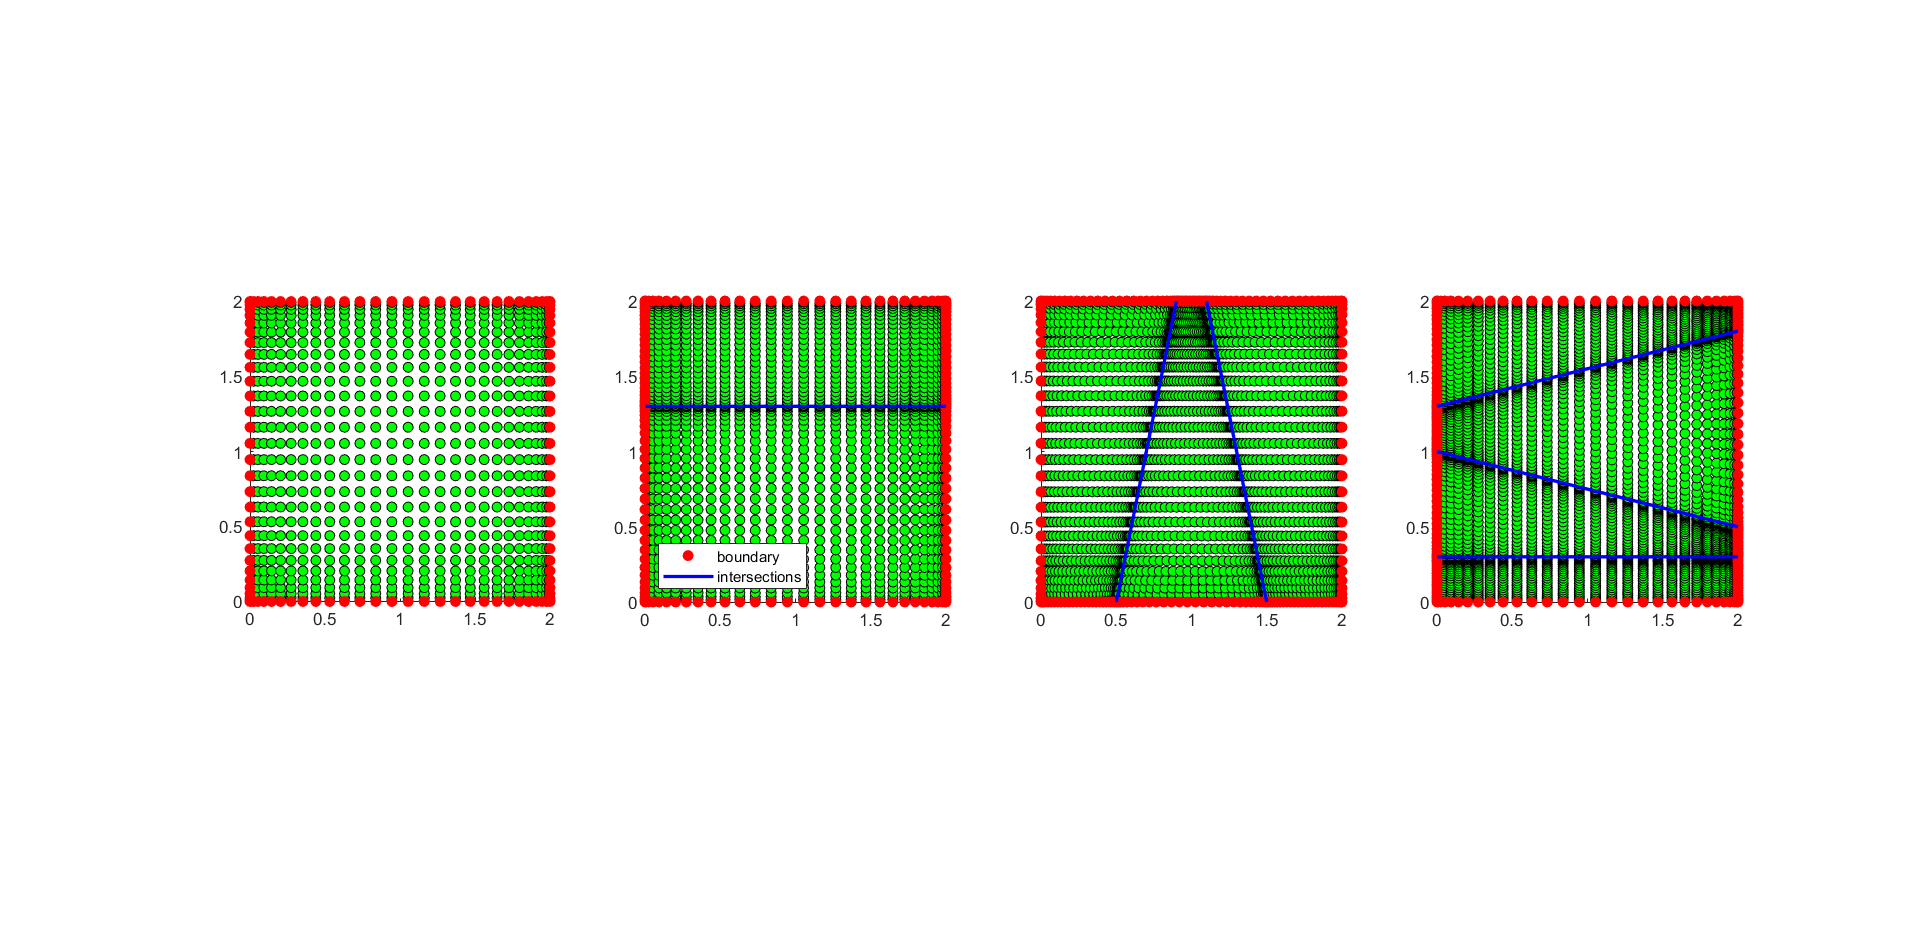
\includegraphics[scale=0.35]{BoxSections.png}
%	\caption{Different discretizations of the box (a - g).} 
%	\label{F2}
%\end{figure}
%\begin{figure}[h]
%	\centering
%	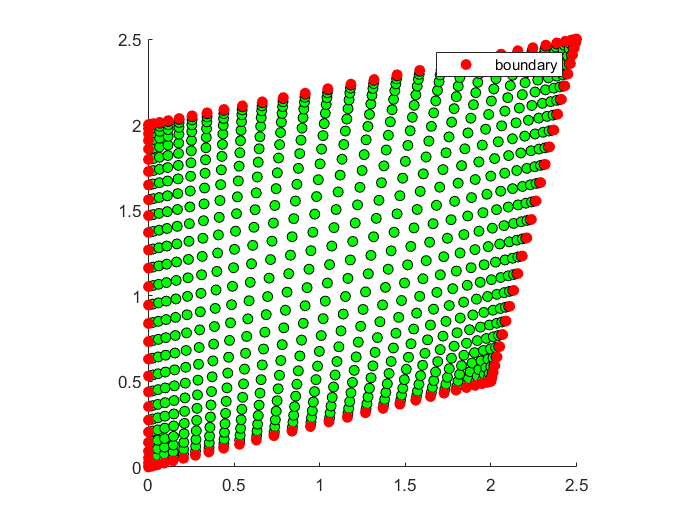
\includegraphics[scale=0.35]{quad.png}
%	\caption{Quadrilateral domain (q).} 
%	\label{F3a}
%\end{figure}
%\begin{figure}[h]
%	\centering
%	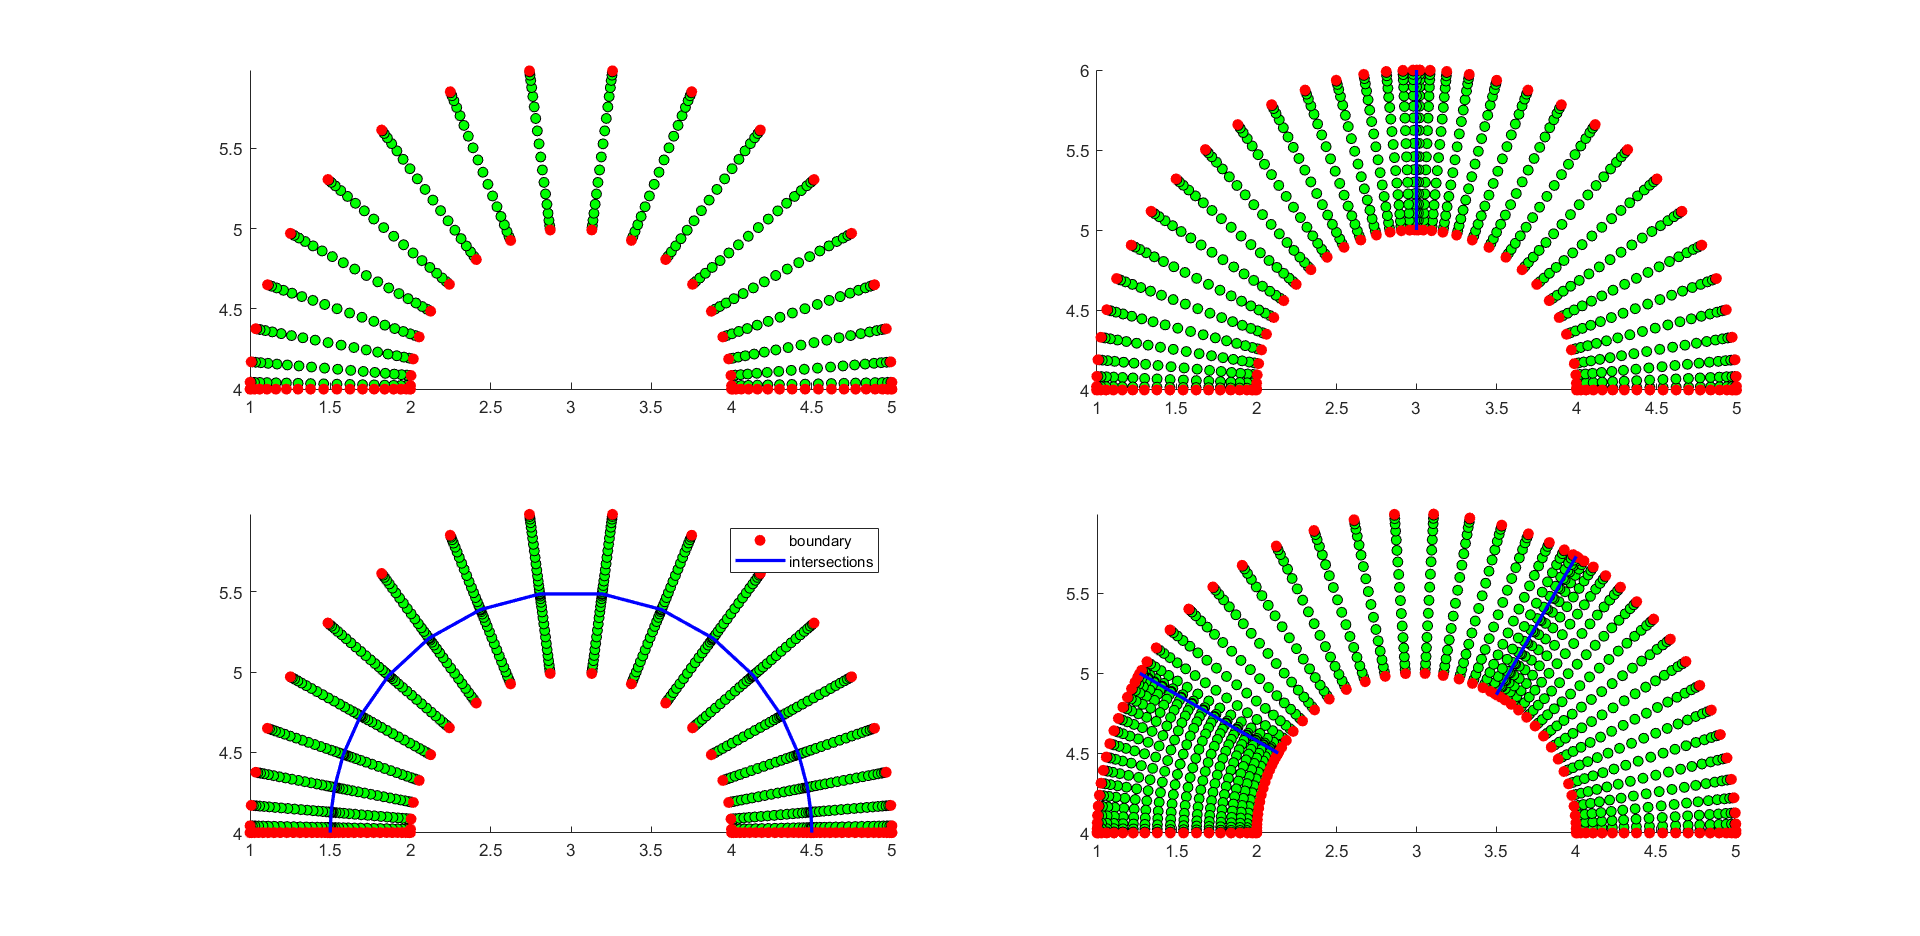
\includegraphics[scale=0.35]{WedgeSections.png}
%	\caption{Different discretizations of the wedge (h - k).} 
%	\label{F4}
%\end{figure}
%
%
%We investigate the accuracy of differentiation, interpolation, integration and convolution comparing different discretizations of the box and a wedge. The different discretizations can be seen in Figures \ref{F2}, \ref{F3a} and \ref{F4}.
%The operations are validated using the exact solution
%\begin{align}\label{eq:exactsol1}
%	\rho &= \exp( \alpha_1  t + \beta_1 y_1 + \beta_2 y_2),\\
%	\nabla \rho &= [\beta_1 \rho, \beta_2 \rho],\notag \\
%	\nabla^2 \rho &= \nabla \cdot \nabla \rho = (\beta_1^2 + \beta_2^2)\rho,\notag
%\end{align}
%where $	\beta_1 = 0.1 $, $\beta_2 = 0.1$, $\alpha_1 = -0.5$.
%
%
%We test each of the operators $\Grad$, $\Div$ and $\Lap$ by computing the error between the numerical and the exact solution
%\begin{align}\label{eq:ErrorMeasure1}
%	\mathcal E_{\text{Abs}} (f)&= \max \max \abs{f_{num} - f_{ex}}\\
%	\mathcal E_{\text{Rel}} (f)&= \frac{\mathcal E_{\text{Abs}}(f) }{ \max \max \abs{f_{ex}}}.
%\end{align}
%The $\Div$ operator is tested by taking the divergence of the exact solution for $\nabla \rho$ and comparing it to the exact solution for $\nabla^2 \rho$. Note that the exact $\nabla \rho$ has to be transformed into polar coordinates first. The solutions can be seen in Tables \ref{Tab:Grad}, \ref{Tab:div} and \ref{Tab:Lap}.
%
%We investigate the functionality of the interpolation matrix by interpolating from the different multishapes onto a uniform grid. This grid is created by setting up a uniform rectangular grid which fully contains the multishape. Then we loop through the shapes and interpolate the test function $\rho$ \eqref{eq:exactsol1} onto the uniform points that lie inside each shape. In the end we discard the points that lie outside the multishape. This causes the final solution on the uniform grid to vary in size, depending on the discretization of the multishape. We test the functionality by comparing the interpolated function values to $\rho$ evaluated on the uniform grid points, using \eqref{eq:ErrorMeasure1}. The results can be seen in Table \ref{Tab:Interp}.
%
%In a second test we interpolate a function $\rho$, \eqref{eq:exactsol1}, computed with $N =50$ on shapes (a) and (h) respectively onto a uniform grid, as described above. Then we compute \eqref{eq:exactsol1} on the multishapes (b), (f), and (g) with $N = 10$, $N = 20$ and $N = 30$. We interpolate this onto the same uniform grid as shape (a) using the physical interpolation function. The values of $\rho$ coming from (a) can be compared with those from (b), (f), and (g) on the uniform grid, using (a) as a reference solution. Similarly, the solution on shape (h) serves as reference solution for multishapes (j) and (k). The errors, computed using \eqref{eq:ErrorMeasure1} can be seen in Table \ref{Tab:InterpComp}.
%
%Finally, we investigate what happens when we consider interpolation to a uniform grid with $N_1 \neq N_2$ for the wedge, when compared to the exact solution on the uniform grid. This is interesting, because when the solution is interpolated onto a uniform grid (in Cartesian coordinates), it is to be expected that more points are needed in the angular direction than in the radial direction, since in Cartesian coordinates points are more densely clustered in radial direction, as can be seen in Figure \ref{F4}. This is indeed what happens, as can be seen in Table \ref{Tab:InterpPol}. We get considerably better results for small $N_1$ than for small $N_2$ and vice versa. We could investigate whether this behaviour changes when we choose a shape with small angle and long radius instead.
%
%We consider a similar approach for testing the convolution matrix. We compute the convolution matrix with $N = 50$ on shape (a) (or (h) respectively) and apply it to the function $\rho$ in equation \eqref{eq:exactsol1}. We then interpolate this onto the other shapes and compute the error \eqref{eq:ErrorMeasure1} with the convolution of $\rho$ on that shape. We use the value of the convolution on a single shape with $N = 50$ as the reference value for the multishape convolution. The results are displayed in Table \ref{Tab:Conv}.
%
%For the integration vector, we compute the integral of $\rho$ on shape (a) and compare this to the integral of $\rho$ on multishapes (b), (f) and (g). We then compare the integral of $\rho$ on the single shape (h) to the one on discretizations (j) and (k). The errors computed with \eqref{eq:ErrorMeasure1} can be seen in Table \ref{Tab:Int}, where again the value of the integral on the single shape is the reference for the multishape integration.
%\begin{table}
\centering
\begin{tabular}{ | c | c | c | c | c | c | c |}
\hline
 & \multicolumn{2}{c|}{$N = 10$}  & \multicolumn{2}{c|}{$N = 20$}  & \multicolumn{2}{c|}{$N = 30$} \\
\hline
 & $\mathcal E_{Abs}$ & $\mathcal E_{Rel}$ & $\mathcal E_{Abs}$ & $\mathcal E_{Rel}$ & $\mathcal E_{Abs}$  & $\mathcal E_{Rel}$ \\
\hline
 a & $\numprint{3.6637e-15}$ & $\numprint{4.0491e-14}$ & $\numprint{4.5158e-14}$ & $\numprint{4.9908e-13}$ & $\numprint{1.0987e-13}$ & $\numprint{1.2143e-12}$ \\
 b & $\numprint{2.5202e-14}$ & $\numprint{2.7853e-13}$ & $\numprint{1.3006e-13}$ & $\numprint{1.4374e-12}$ & $\numprint{3.9264e-13}$ & $\numprint{4.3394e-12}$ \\
 c & $\numprint{3.5680e-14}$ & $\numprint{3.9432e-13}$ & $\numprint{2.7724e-13}$ & $\numprint{3.0639e-12}$ & $\numprint{1.0356e-12}$ & $\numprint{1.1445e-11}$ \\
 d & $\numprint{7.3080e-14}$ & $\numprint{8.0766e-13}$ & $\numprint{6.0429e-13}$ & $\numprint{6.6785e-12}$ & $\numprint{1.2559e-12}$ & $\numprint{1.3880e-11}$ \\
 e & $\numprint{3.1912e-14}$ & $\numprint{3.5268e-13}$ & $\numprint{2.0508e-13}$ & $\numprint{2.2665e-12}$ & $\numprint{6.5671e-13}$ & $\numprint{7.2578e-12}$ \\
 f & $\numprint{5.7149e-14}$ & $\numprint{6.3159e-13}$ & $\numprint{4.4410e-13}$ & $\numprint{4.9081e-12}$ & $\numprint{1.7717e-12}$ & $\numprint{1.9580e-11}$ \\
 g & $\numprint{1.3947e-14}$ & $\numprint{1.5414e-13}$ & $\numprint{9.5771e-14}$ & $\numprint{1.0584e-12}$ & $\numprint{2.6459e-13}$ & $\numprint{2.9242e-12}$ \\
 h & $\numprint{3.1143e-5}$ & $\numprint{1.3588e-4}$ & $\numprint{1.3522e-11}$ & $\numprint{5.9203e-11}$ & $\numprint{4.0515e-13}$ & $\numprint{1.7705e-12}$ \\
 i & $\numprint{1.3490e-7}$ & $\numprint{5.9567e-7}$ & $\numprint{2.4433e-13}$ & $\numprint{1.0689e-12}$ & $\numprint{4.5003e-13}$ & $\numprint{1.9658e-12}$ \\
 j & $\numprint{3.1143e-5}$ & $\numprint{1.3588e-4}$ & $\numprint{1.3522e-11}$ & $\numprint{5.9203e-11}$ & $\numprint{9.8901e-13}$ & $\numprint{4.3219e-12}$ \\
 k & $\numprint{9.8299e-8}$ & $\numprint{4.2888e-7}$ & $\numprint{3.1769e-13}$ & $\numprint{1.3866e-12}$ & $\numprint{8.6467e-13}$ & $\numprint{3.7732e-12}$ \\
\hline
\end{tabular}
\caption{Table $\Grad$}
\label{Tab:Grad}
\end{table}
%\begin{table}
\centering
\begin{tabular}{ | c | c | c | c | c | c | c |}
\hline
 & \multicolumn{2}{c|}{$N = 10$}  & \multicolumn{2}{c|}{$N = 20$}  & \multicolumn{2}{c|}{$N = 30$} \\
\hline
 & $\mathcal E_{Abs}$ & $\mathcal E_{Rel}$ & $\mathcal E_{Abs}$ & $\mathcal E_{Rel}$ & $\mathcal E_{Abs}$  & $\mathcal E_{Rel}$ \\
\hline
 a & $\numprint{8.3267e-16}$ & $\numprint{4.6012e-14}$ & $\numprint{4.8798e-15}$ & $\numprint{2.6965e-13}$ & $\numprint{1.2278e-14}$ & $\numprint{6.7849e-13}$ \\
 b & $\numprint{2.9594e-15}$ & $\numprint{1.6353e-13}$ & $\numprint{1.3121e-14}$ & $\numprint{7.2507e-13}$ & $\numprint{4.0837e-14}$ & $\numprint{2.2566e-12}$ \\
 c & $\numprint{8.3614e-15}$ & $\numprint{4.6204e-13}$ & $\numprint{2.8682e-14}$ & $\numprint{1.5849e-12}$ & $\numprint{1.0649e-13}$ & $\numprint{5.8845e-12}$ \\
 d & $\numprint{7.9138e-15}$ & $\numprint{4.3731e-13}$ & $\numprint{4.2664e-14}$ & $\numprint{2.3575e-12}$ & $\numprint{9.6187e-14}$ & $\numprint{5.3152e-12}$ \\
 e & $\numprint{3.6846e-15}$ & $\numprint{2.0360e-13}$ & $\numprint{2.1975e-14}$ & $\numprint{1.2143e-12}$ & $\numprint{6.9682e-14}$ & $\numprint{3.8505e-12}$ \\
 f & $\numprint{9.7717e-15}$ & $\numprint{5.3997e-13}$ & $\numprint{6.4991e-14}$ & $\numprint{3.5913e-12}$ & $\numprint{1.3360e-13}$ & $\numprint{7.3824e-12}$ \\
 g & $\numprint{3.0878e-15}$ & $\numprint{1.7063e-13}$ & $\numprint{1.0623e-14}$ & $\numprint{5.8704e-13}$ & $\numprint{3.3662e-14}$ & $\numprint{1.8601e-12}$ \\
 h & $\numprint{5.2272e-5}$ & $\numprint{1.6127e-3}$ & $\numprint{3.4844e-11}$ & $\numprint{1.0758e-9}$ & $\numprint{5.3096e-14}$ & $\numprint{1.6387e-12}$ \\
 i & $\numprint{9.2692e-8}$ & $\numprint{2.8672e-6}$ & $\numprint{3.2897e-14}$ & $\numprint{1.0155e-12}$ & $\numprint{6.4497e-14}$ & $\numprint{1.9903e-12}$ \\
 j & $\numprint{5.2272e-5}$ & $\numprint{1.6127e-3}$ & $\numprint{3.4852e-11}$ & $\numprint{1.0761e-9}$ & $\numprint{1.3768e-13}$ & $\numprint{4.2490e-12}$ \\
 k & $\numprint{8.4307e-8}$ & $\numprint{2.6010e-6}$ & $\numprint{4.5634e-14}$ & $\numprint{1.4080e-12}$ & $\numprint{9.0605e-14}$ & $\numprint{2.7954e-12}$ \\
\hline
\end{tabular}
\caption{Table $\Div$}
\label{Tab:div}
\end{table}
%\begin{table}
\centering
\begin{tabular}{ | c | c | c | c | c | c | c |}
\hline
 & \multicolumn{2}{c|}{$N = 10$}  & \multicolumn{2}{c|}{$N = 20$}  & \multicolumn{2}{c|}{$N = 30$} \\
\hline
 & $\mathcal E_{Abs}$ & $\mathcal E_{Rel}$ & $\mathcal E_{Abs}$ & $\mathcal E_{Rel}$ & $\mathcal E_{Abs}$  & $\mathcal E_{Rel}$ \\
\hline
 a & $\numprint{1.7055e-13}$ & $\numprint{9.4244e-12}$ & $\numprint{4.7951e-12}$ & $\numprint{2.6497e-10}$ & $\numprint{2.5029e-11}$ & $\numprint{1.3831e-9}$ \\
 b & $\numprint{1.3937e-12}$ & $\numprint{7.7015e-11}$ & $\numprint{4.4301e-11}$ & $\numprint{2.4480e-9}$ & $\numprint{1.2869e-10}$ & $\numprint{7.1114e-9}$ \\
 c & $\numprint{7.7744e-12}$ & $\numprint{4.2960e-10}$ & $\numprint{3.8083e-10}$ & $\numprint{2.1044e-8}$ & $\numprint{3.8902e-9}$ & $\numprint{2.1497e-7}$ \\
 d & $\numprint{1.4964e-11}$ & $\numprint{8.2688e-10}$ & $\numprint{5.5707e-10}$ & $\numprint{3.0783e-8}$ & $\numprint{1.6726e-9}$ & $\numprint{9.2426e-8}$ \\
 e & $\numprint{4.2647e-12}$ & $\numprint{2.3566e-10}$ & $\numprint{1.0580e-10}$ & $\numprint{5.8462e-9}$ & $\numprint{1.0035e-9}$ & $\numprint{5.5450e-8}$ \\
 f & $\numprint{1.4029e-11}$ & $\numprint{7.7521e-10}$ & $\numprint{5.8611e-10}$ & $\numprint{3.2388e-8}$ & $\numprint{3.0143e-9}$ & $\numprint{1.6657e-7}$ \\
 g & $\numprint{9.4664e-13}$ & $\numprint{5.2310e-11}$ & $\numprint{3.5819e-11}$ & $\numprint{1.9793e-9}$ & $\numprint{1.4403e-10}$ & $\numprint{7.9586e-9}$ \\
 h & $\numprint{5.3665e-4}$ & $\numprint{1.6556e-2}$ & $\numprint{1.0457e-9}$ & $\numprint{3.2287e-8}$ & $\numprint{1.7551e-10}$ & $\numprint{5.4167e-9}$ \\
 i & $\numprint{4.6482e-6}$ & $\numprint{1.4378e-4}$ & $\numprint{5.0420e-11}$ & $\numprint{1.5565e-9}$ & $\numprint{2.3952e-10}$ & $\numprint{7.3915e-9}$ \\
 j & $\numprint{5.3665e-4}$ & $\numprint{1.6556e-2}$ & $\numprint{1.0223e-9}$ & $\numprint{3.1565e-8}$ & $\numprint{7.2370e-10}$ & $\numprint{2.2335e-8}$ \\
 k & $\numprint{3.3996e-6}$ & $\numprint{1.0488e-4}$ & $\numprint{1.0291e-10}$ & $\numprint{3.1753e-9}$ & $\numprint{4.0443e-10}$ & $\numprint{1.2478e-8}$ \\
\hline
\end{tabular}
\caption{Table $\Lap$}
\label{Tab:Lap}
\end{table}
%\begin{table}
\centering
\begin{tabular}{ | c | c | c | c | c | c | c |}
\hline
 & \multicolumn{2}{c|}{$N = 10$}  & \multicolumn{2}{c|}{$N = 20$}  & \multicolumn{2}{c|}{$N = 30$} \\
\hline
 & $\mathcal E_{Abs}$ & $\mathcal E_{Rel}$ & $\mathcal E_{Abs}$ & $\mathcal E_{Rel}$& $\mathcal E_{Abs}$  & $\mathcal E_{Rel}$ \\
\hline
 a & $\numprint{9.9920e-16}$ & $\numprint{1.1043e-15}$ & $\numprint{1.1102e-15}$ & $\numprint{1.2270e-15}$ & $\numprint{1.9984e-15}$ & $\numprint{2.2086e-15}$ \\
 b & $\numprint{8.8818e-16}$ & $\numprint{9.8159e-16}$ & $\numprint{1.5543e-15}$ & $\numprint{1.7178e-15}$ & $\numprint{1.8874e-15}$ & $\numprint{2.0859e-15}$ \\
 c & $\numprint{8.8818e-16}$ & $\numprint{9.8159e-16}$ & $\numprint{1.6653e-15}$ & $\numprint{1.8405e-15}$ & $\numprint{2.2204e-15}$ & $\numprint{2.4540e-15}$ \\
 d & $\numprint{8.8818e-16}$ & $\numprint{9.8159e-16}$ & $\numprint{1.9984e-15}$ & $\numprint{2.2086e-15}$ & $\numprint{2.6645e-15}$ & $\numprint{2.9448e-15}$ \\
 e & $\numprint{8.8818e-16}$ & $\numprint{9.8159e-16}$ & $\numprint{1.4433e-15}$ & $\numprint{1.5951e-15}$ & $\numprint{2.6645e-15}$ & $\numprint{2.9448e-15}$ \\
 f & $\numprint{1.2212e-15}$ & $\numprint{1.3497e-15}$ & $\numprint{1.6653e-15}$ & $\numprint{1.8405e-15}$ & $\numprint{2.8866e-15}$ & $\numprint{3.1902e-15}$ \\
 g & $\numprint{8.8818e-16}$ & $\numprint{9.8159e-16}$ & $\numprint{1.8874e-15}$ & $\numprint{2.0859e-15}$ & $\numprint{2.5535e-15}$ & $\numprint{2.8221e-15}$ \\
 h & $\numprint{4.6655e-6}$ & $\numprint{2.8922e-6}$ & $\numprint{7.9314e-13}$ & $\numprint{4.9000e-13}$ & $\numprint{2.6645e-15}$ & $\numprint{1.6450e-15}$ \\
 i & $\numprint{1.1935e-8}$ & $\numprint{7.3650e-9}$ & $\numprint{3.3307e-15}$ & $\numprint{2.0553e-15}$ & $\numprint{3.1086e-15}$ & $\numprint{1.9183e-15}$ \\
 j & $\numprint{4.6655e-6}$ & $\numprint{2.8922e-6}$ & $\numprint{7.9226e-13}$ & $\numprint{4.8945e-13}$ & $\numprint{4.2188e-15}$ & $\numprint{2.6047e-15}$ \\
 k & $\numprint{7.7730e-9}$ & $\numprint{4.8017e-9}$ & $\numprint{2.2204e-15}$ & $\numprint{1.3705e-15}$ & $\numprint{4.4409e-15}$ & $\numprint{2.7405e-15}$ \\
\hline
\end{tabular}
\caption{Table Interp}
\label{Tab:Interp}
\end{table}
%\begin{table}
\centering
\begin{tabular}{ | c | c | c | c | c | c | c |}
\hline
 & \multicolumn{2}{c|}{$N = 10$}  & \multicolumn{2}{c|}{$N = 20$}  & \multicolumn{2}{c|}{$N = 30$} \\
\hline
 & $\mathcal E_{Abs}$ & $\mathcal E_{Rel}$ & $\mathcal E_{Abs}$ & $\mathcal E_{Rel}$ & $\mathcal E_{Abs}$  & $\mathcal E_{Rel}$ \\
\hline
 b & $\numprint{2.3315e-15}$ & $\numprint{2.5767e-15}$ & $\numprint{2.3315e-15}$ & $\numprint{2.5767e-15}$ & $\numprint{3.2196e-15}$ & $\numprint{3.5583e-15}$ \\
 c & $\numprint{2.4425e-15}$ & $\numprint{2.6994e-15}$ & $\numprint{2.8866e-15}$ & $\numprint{3.1902e-15}$ & $\numprint{2.5535e-15}$ & $\numprint{2.8221e-15}$ \\
 d & $\numprint{2.3315e-15}$ & $\numprint{2.5767e-15}$ & $\numprint{3.2196e-15}$ & $\numprint{3.5583e-15}$ & $\numprint{3.3307e-15}$ & $\numprint{3.6810e-15}$ \\
 e & $\numprint{2.3315e-15}$ & $\numprint{2.5767e-15}$ & $\numprint{2.6645e-15}$ & $\numprint{2.9448e-15}$ & $\numprint{2.8866e-15}$ & $\numprint{3.1902e-15}$ \\
 f & $\numprint{2.2204e-15}$ & $\numprint{2.4540e-15}$ & $\numprint{2.7756e-15}$ & $\numprint{3.0675e-15}$ & $\numprint{3.2196e-15}$ & $\numprint{3.5583e-15}$ \\
 g & $\numprint{2.6645e-15}$ & $\numprint{2.9448e-15}$ & $\numprint{2.9976e-15}$ & $\numprint{3.3129e-15}$ & $\numprint{3.6637e-15}$ & $\numprint{4.0491e-15}$ \\
 i & $\numprint{1.1886e-8}$ & $\numprint{7.3362e-9}$ & $\numprint{5.1070e-15}$ & $\numprint{3.1520e-15}$ & $\numprint{6.4393e-15}$ & $\numprint{3.9742e-15}$ \\
 j & $\numprint{4.8940e-6}$ & $\numprint{3.0205e-6}$ & $\numprint{8.1379e-13}$ & $\numprint{5.0226e-13}$ & $\numprint{4.6629e-15}$ & $\numprint{2.8779e-15}$ \\
 k & $\numprint{7.8923e-9}$ & $\numprint{4.8710e-9}$ & $\numprint{5.1070e-15}$ & $\numprint{3.1520e-15}$ & $\numprint{5.1070e-15}$ & $\numprint{3.1520e-15}$ \\
\hline
\end{tabular}
\caption{Table Interp Compare}
\label{Tab:InterpComp}
\end{table}
%\begin{table}
\centering
\begin{tabular}{ | c | c | c | c | c | c | c |}
\hline
 & $N_1 = 20$ & $N_1 = 20$& $N_1 = 5$& $N_1 = 10$& $N_1 = 30$  & $N_1 = 20$ \\
\hline
 & $N_2 = 10$ & $ N_2 = 15$ & $ N_2 = 20$ & $ N_2 = 20$ & $ N_2 = 20$  & $ N_2 = 30$ \\
\hline
 h & $\numprint{2.8922e-6}$ & $\numprint{5.1117e-10}$ & $\numprint{1.5795e-9}$ & $\numprint{4.8973e-13}$ & $\numprint{4.9000e-13}$ & $\numprint{1.5080e-15}$ \\
 i & $\numprint{7.3650e-9}$ & $\numprint{1.6031e-14}$ & $\numprint{1.5807e-9}$ & $\numprint{1.2332e-15}$ & $\numprint{1.9183e-15}$ & $\numprint{2.4663e-15}$ \\
 j & $\numprint{2.8922e-6}$ & $\numprint{5.1117e-10}$ & $\numprint{5.1835e-11}$ & $\numprint{4.8959e-13}$ & $\numprint{4.8986e-13}$ & $\numprint{1.9192e-15}$ \\
 k & $\numprint{4.8017e-9}$ & $\numprint{7.6215e-14}$ & $\numprint{1.5808e-9}$ & $\numprint{1.2334e-15}$ & $\numprint{2.4668e-15}$ & $\numprint{2.0554e-15}$ \\
\hline
\end{tabular}
\caption{Table Comparing interpolation errors on wedges, when $N_1 \neq N_2$.}
\label{Tab:InterpPol}
\end{table}
%\begin{table}
\centering
\begin{tabular}{ | c | c || c | c | c | c | c ||}
\hline
 & A.E. $ N=10$ & R.E. $N=10$ & A.E. $N = 20$ & R.E. $N = 20$ & A.E. $N=30$  & R.E. $N=30$ \\
\hline
\hline
 b & $\numprint{9.1924e-8}$ & $\numprint{5.5907e-8}$ & $\numprint{7.5495e-15}$ & $\numprint{4.5500e-15}$ & $\numprint{8.2157e-15}$ & $\numprint{4.9463e-15}$ \\
 f & $\numprint{1.4109e-8}$ & $\numprint{8.5341e-9}$ & $\numprint{8.2157e-15}$ & $\numprint{4.9497e-15}$ & $\numprint{1.9984e-14}$ & $\numprint{1.2033e-14}$ \\
 g & $\numprint{1.9228e-10}$ & $\numprint{1.1579e-10}$ & $\numprint{9.7700e-15}$ & $\numprint{5.8815e-15}$ & $\numprint{1.5543e-14}$ & $\numprint{9.3564e-15}$ \\
 j & $\numprint{1.6310e-3}$ & $\numprint{6.6333e-4}$ & $\numprint{5.0919e-8}$ & $\numprint{2.0616e-8}$ & $\numprint{8.9782e-12}$ & $\numprint{3.6342e-12}$ \\
 k & $\numprint{2.7196e-6}$ & $\numprint{1.1056e-6}$ & $\numprint{1.7668e-12}$ & $\numprint{7.1588e-13}$ & $\numprint{2.9310e-14}$ & $\numprint{1.1870e-14}$ \\
\hline
\end{tabular}
\caption{Table Conv}
\label{Tab:Conv}
\end{table}
%\begin{table}
\centering
\begin{tabular}{ | c | c || c | c | c | c | c ||}
\hline
 & A.E. $ N=10$ & R.E. $N=10$ & A.E. $N = 20$ & R.E. $N = 20$ & A.E. $N=30$  & R.E. $N=30$ \\
\hline
\hline
 b & $\numprint{0.0000e+00}$ & $\numprint{0.0000e+00}$ & $\numprint{4.4409e-16}$ & $\numprint{1.4937e-16}$ & $\numprint{8.8818e-16}$ & $\numprint{2.9873e-16}$ \\
 f & $\numprint{0.0000e+00}$ & $\numprint{0.0000e+00}$ & $\numprint{0.0000e+00}$ & $\numprint{0.0000e+00}$ & $\numprint{8.8818e-16}$ & $\numprint{2.9873e-16}$ \\
 g & $\numprint{0.0000e+00}$ & $\numprint{0.0000e+00}$ & $\numprint{4.4409e-16}$ & $\numprint{1.4937e-16}$ & $\numprint{8.8818e-16}$ & $\numprint{2.9873e-16}$ \\
 j & $\numprint{2.4085e-8}$ & $\numprint{3.7621e-9}$ & $\numprint{1.7764e-15}$ & $\numprint{2.7746e-16}$ & $\numprint{2.6645e-15}$ & $\numprint{4.1620e-16}$ \\
 k & $\numprint{2.7334e-11}$ & $\numprint{4.2695e-12}$ & $\numprint{1.7764e-15}$ & $\numprint{2.7746e-16}$ & $\numprint{1.7764e-15}$ & $\numprint{2.7746e-16}$ \\
\hline
\end{tabular}
\caption{Table Int}
\label{Tab:Int}
\end{table}


\subsubsection{Exact Tests}
The solution to known testproblems with Dirichlet and no-flux boundary conditions are considered in this section. The errors are calculated as an $l_2$ error in space and an $l_\infty$ error in time.
\subsubsection*{Exact Tests - Dirichlet Conditions}
(MS\_TestJonnaADExactDisectBoxes and MS\_TestJonnaADExactDisectBoxesPart2\\ and MS\_TestJonnaADExactDisectWedges)
Several examples are run, using exact solutions, to validate the multishape code. This is done using an exact solution to the advection diffusion equation on an infinite domain, so that Dirichlet boundary conditions can be applied, by matching the value of the exact solution on the boundary of the multishape.
The exact solution is \cite{Hutomo_2019}
\begin{align}\label{eq:DirichletExactSol}
	\rho &= \exp(\alpha t + \beta_1 y_1 + \beta_2 y_2)\\
	\mathbf v &= \left(\beta_1 - \frac{\alpha}{2 \beta_1} + p_1\exp(-\beta_1 y_1) , \beta_2 - \frac{\alpha}{2 \beta_2} + p_2\exp(-\beta_2 y_2) \right),\notag
\end{align}
where $\beta_1 = 0.1$, $\beta_2 = 0.1$, $\alpha = -0.5$, $p_1 = -1$ and $p_2 = 1$.
We compare the exact solution on a box of dimensions $[0,2] \times [0,2] $ with different discretizations of the box using multishape, signified by letters (a) to (g), see Figure \ref{F2}. Each of the shapes are discretized with $N = 10$, $N = 20$ and $N = 30$ points in each spatial direction, which means that the dissected box has more points in total than the original box. The ODE solver tolerances are $10^{-9}$. The solution can be seen in Figure \ref{F3}. The question is whether the results of the PDE on the box and the different discretizations of the box have a similar error when compared to the exact solution. The absolute and relative errors, $\mathcal E_{Abs}$ and $\mathcal E_{Rel}$, are measured in an $l_2$ norm in space and an $l_\infty$ norm in time and are displayed in Table \ref{Tab:DirichletEx1}. The errors for the non-rectangular quadrilateral, which is shown in Figure \ref{F3a}, are displayed on the row with the letter (q). 


	\begin{figure}[h]
		\centering
		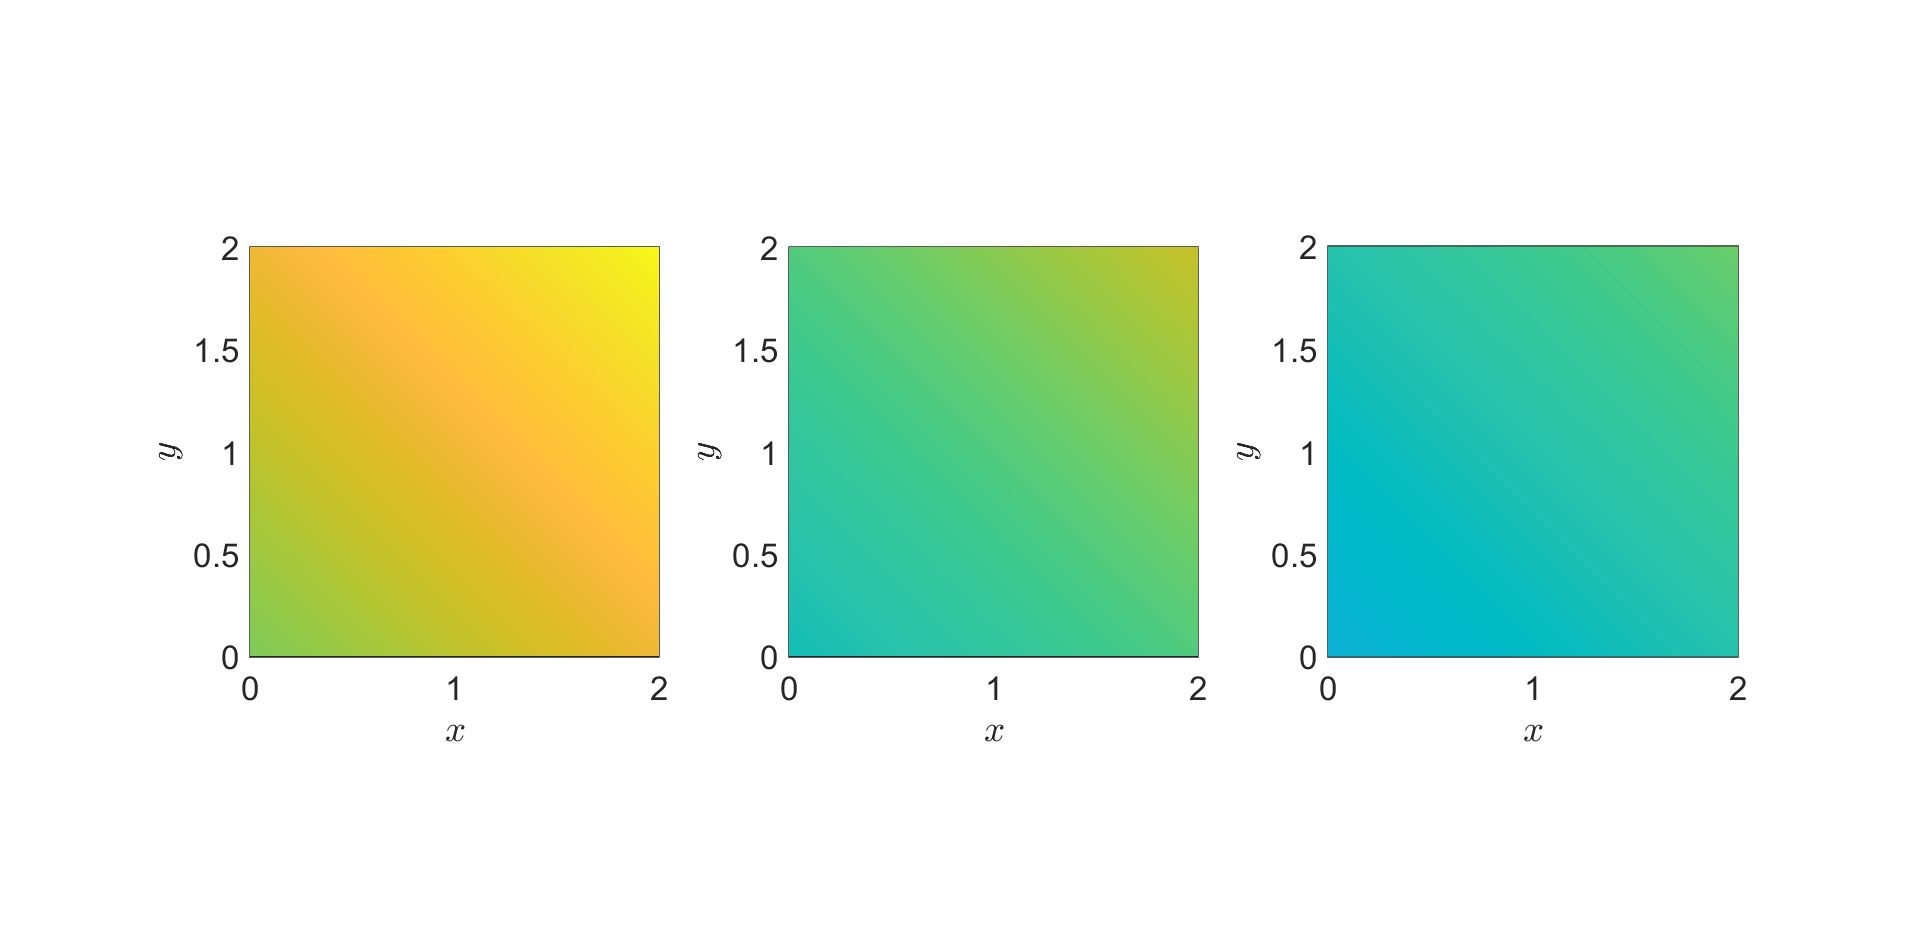
\includegraphics[scale=0.35]{boxEx.png}
		\caption{Exact solution on the box.} 
		\label{F3}
	\end{figure}


The same test can be done for a wedge. Here, a single wedge and discretized versions are considered, denoted by (h) to (k), see Figure \ref{F4}. Table \ref{Tab:DirichletEx1} also shows the errors measured against the exact solution for different discretizations of the wedge, for $N = 10$, $N = 20$ and $N = 30$. The solution can be seen in Figure \ref{F5}.


\begin{figure}[h]
	\centering
	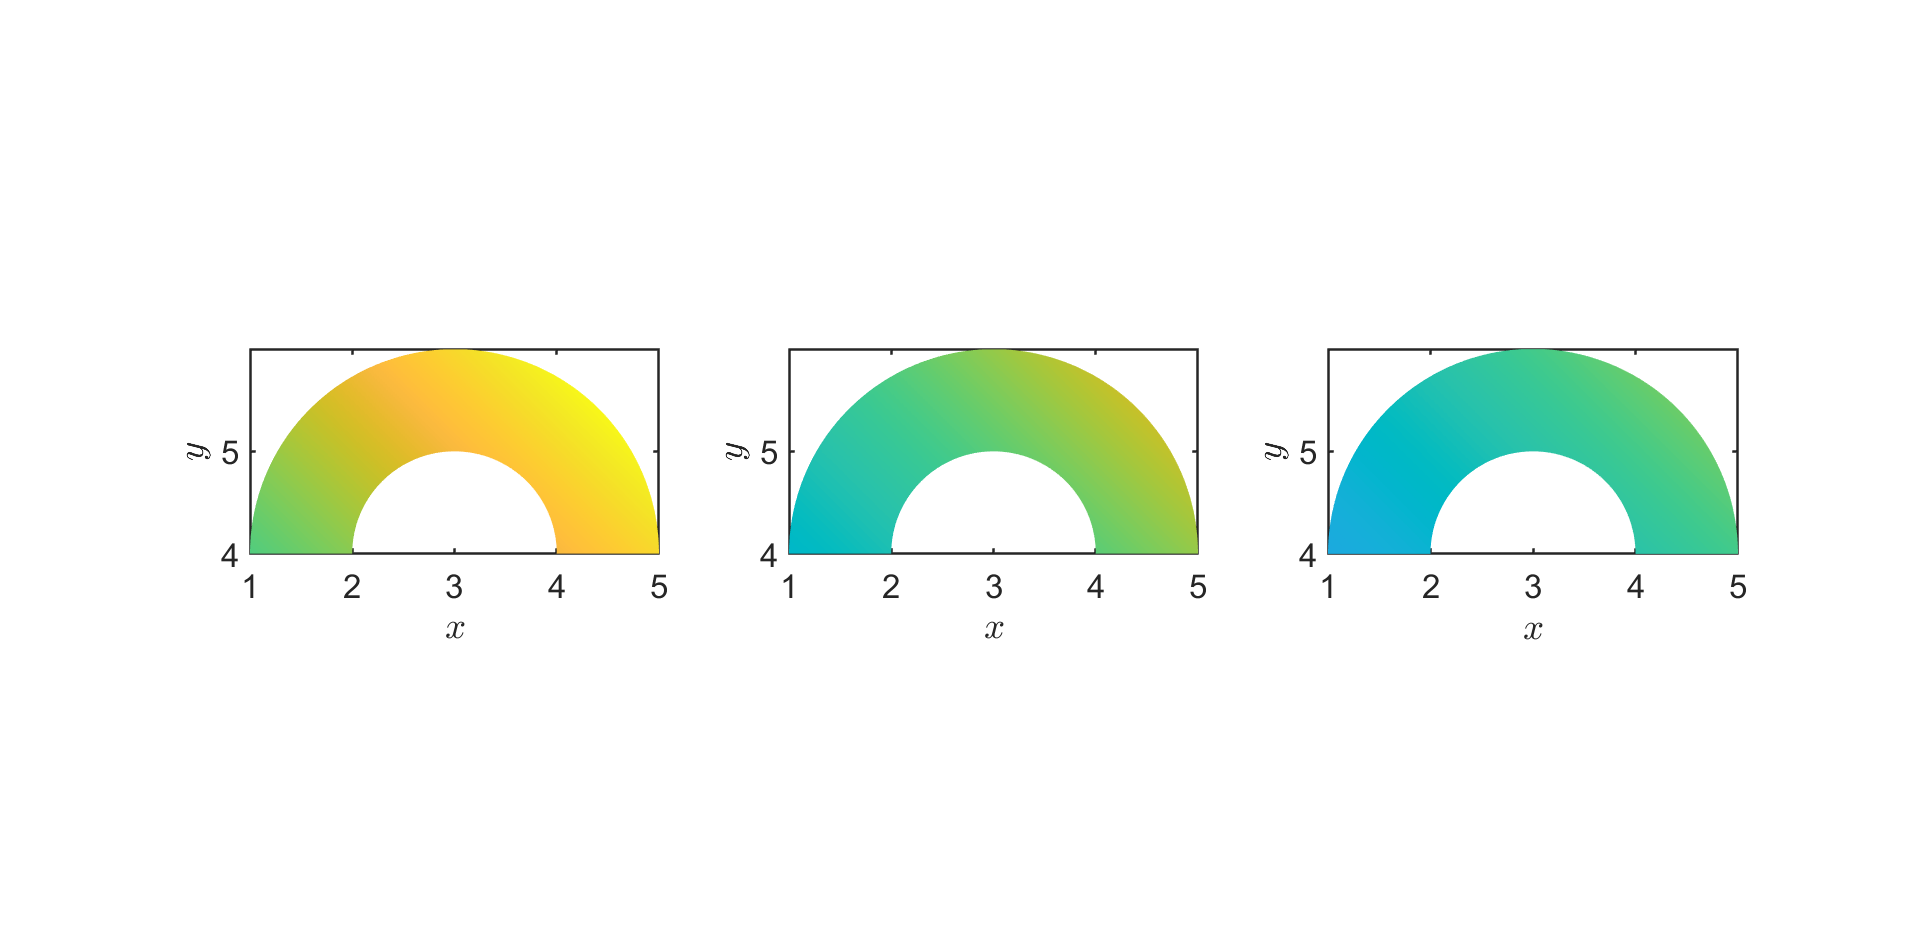
\includegraphics[scale=0.35]{wedgeEx.png}
	\caption{Exact solution on the wedge.} 
	\label{F5}
\end{figure}

Next the advection diffusion equation is solved on a multishape which is composed of four quadrilaterals, see Figure \ref{F6}.  The same is done for a second example involving a wedge, see Figure \ref{F7}.  The errors, as compared to the exact solution \eqref{eq:DirichletExactSol}, are displayed in Table \ref{Tab:DirichletEx1MS}. There, the first multishape is denoted ms1 and the second ms2.
\begin{figure}[h]
	\centering
	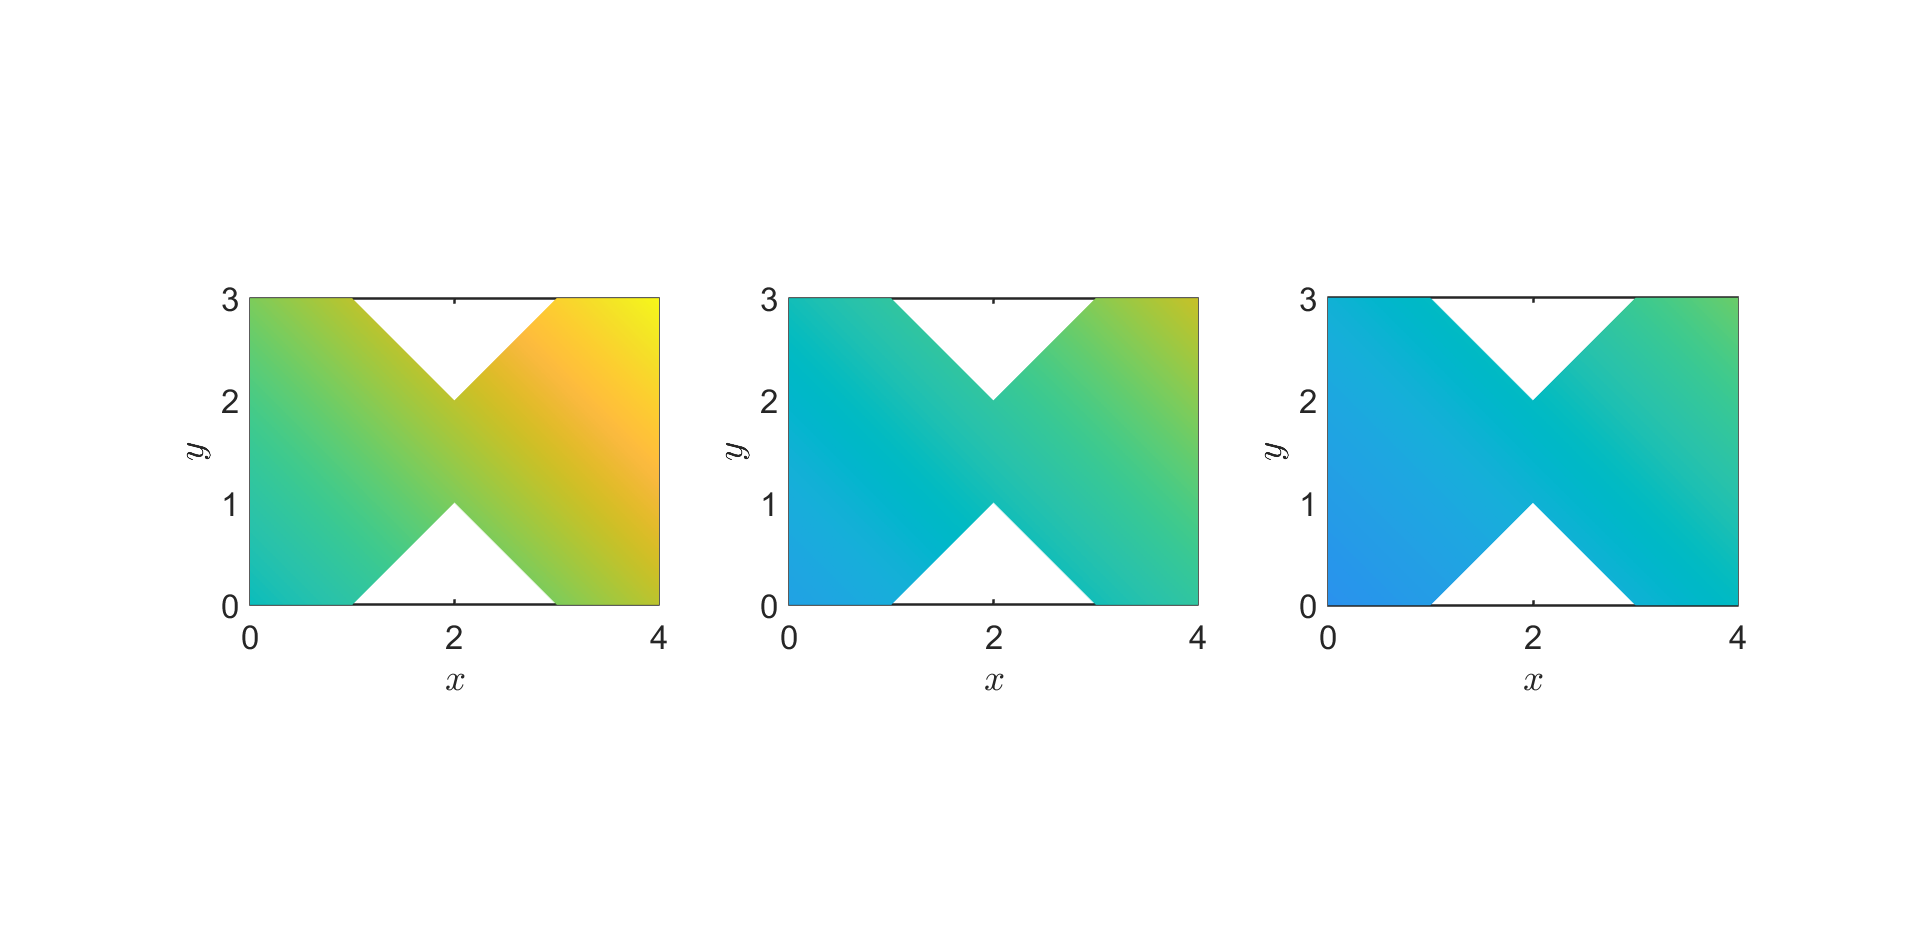
\includegraphics[scale=0.35]{example1.png}
	\caption{Example 1 multishape} 
	\label{F6}
\end{figure}


\begin{figure}[h]
	\centering
	\includegraphics[scale=0.35]{example2.png}
	\caption{Example 2 multishape} 
	\label{F7}
\end{figure}

\begin{table}
\centering
\begin{tabular}{ | c | c | c | c | c | c | c |}
\hline
 & \multicolumn{2}{c|}{$N = 10$}  & \multicolumn{2}{c|}{$N = 20$}  & \multicolumn{2}{c|}{$N = 30$} \\
\hline
 & $\mathcal E_{Abs}$ & $\mathcal E_{Rel}$ & $\mathcal E_{Abs}$ & $\mathcal E_{Rel}$ & $\mathcal E_{Abs}$  & $\mathcal E_{Rel}$ \\
\hline
 a & $\numprint{2.5869e-7}$ & $\numprint{1.0894e-9}$ & $\numprint{2.2063e-7}$ & $\numprint{1.1235e-9}$ & $\numprint{2.1913e-7}$ & $\numprint{1.1159e-9}$ \\
 b & $\numprint{3.4991e-7}$ & $\numprint{1.1308e-9}$ & $\numprint{3.2073e-7}$ & $\numprint{1.1377e-9}$ & $\numprint{3.1877e-7}$ & $\numprint{1.1307e-9}$ \\
 c & $\numprint{4.1386e-7}$ & $\numprint{1.1596e-9}$ & $\numprint{3.9107e-7}$ & $\numprint{1.1500e-9}$ & $\numprint{3.8858e-7}$ & $\numprint{1.1426e-9}$ \\
 d & $\numprint{4.2622e-7}$ & $\numprint{1.0268e-9}$ & $\numprint{3.9019e-7}$ & $\numprint{1.0026e-9}$ & $\numprint{3.8768e-7}$ & $\numprint{9.9616e-10}$ \\
 e & $\numprint{4.4595e-7}$ & $\numprint{1.0704e-9}$ & $\numprint{3.3852e-7}$ & $\numprint{9.8259e-10}$ & $\numprint{3.3718e-7}$ & $\numprint{1.0085e-9}$ \\
 f & $\numprint{4.1985e-7}$ & $\numprint{1.0275e-9}$ & $\numprint{4.2547e-7}$ & $\numprint{1.0412e-9}$ & $\numprint{4.2291e-7}$ & $\numprint{1.0350e-9}$ \\
 g & $\numprint{5.0161e-7}$ & $\numprint{1.1254e-9}$ & $\numprint{4.4470e-7}$ & $\numprint{1.1323e-9}$ & $\numprint{4.3978e-7}$ & $\numprint{1.1198e-9}$ \\
 q & $\numprint{2.4145e-7}$ & $\numprint{1.0389e-9}$ & $\numprint{2.2844e-7}$ & $\numprint{1.1160e-9}$ & $\numprint{2.2505e-7}$ & $\numprint{1.0995e-9}$ \\
 h & $\numprint{1.8507e-3}$ & $\numprint{4.4410e-6}$ & $\numprint{3.1141e-7}$ & $\numprint{7.4763e-10}$ & $\numprint{2.7613e-7}$ & $\numprint{7.5178e-10}$ \\
 i & $\numprint{3.4678e-6}$ & $\numprint{6.5183e-9}$ & $\numprint{3.9525e-7}$ & $\numprint{7.5983e-10}$ & $\numprint{3.8485e-7}$ & $\numprint{7.4376e-10}$ \\
 j & $\numprint{2.6220e-3}$ & $\numprint{4.4489e-6}$ & $\numprint{4.2335e-7}$ & $\numprint{7.4943e-10}$ & $\numprint{3.8922e-7}$ & $\numprint{7.5064e-10}$ \\
 k & $\numprint{2.6814e-6}$ & $\numprint{4.0877e-9}$ & $\numprint{4.4144e-7}$ & $\numprint{7.0896e-10}$ & $\numprint{4.3211e-7}$ & $\numprint{6.9682e-10}$ \\
\hline
\end{tabular}
\caption{Table Dirichlet Exact Solution 1}
\label{Tab:DirichletEx1}
\end{table}
\begin{table}
\centering
\begin{tabular}{ | c | c | c | c | c | c | c |}
\hline
 & \multicolumn{2}{c|}{$N = 10$}  & \multicolumn{2}{c|}{$N = 20$}  & \multicolumn{2}{c|}{$N = 30$} \\
\hline
 & $\mathcal E_{Abs}$ & $\mathcal E_{Rel}$ & $\mathcal E_{Abs}$ & $\mathcal E_{Rel}$ & $\mathcal E_{Abs}$  & $\mathcal E_{Rel}$ \\
\hline
 ms1 & $\numprint{5.9588e-7}$ & $\numprint{1.3030e-9}$ & $\numprint{6.1246e-7}$ & $\numprint{1.3259e-9}$ & $\numprint{6.0034e-7}$ & $\numprint{1.2997e-9}$ \\
 ms2 & $\numprint{1.6829e-3}$ & $\numprint{3.6591e-6}$ & $\numprint{3.7239e-7}$ & $\numprint{8.9375e-10}$ & $\numprint{3.7589e-7}$ & $\numprint{8.9532e-10}$ \\
\hline
\end{tabular}
\caption{Table Dirichlet Exact Solution 1 on two multishapes}
\label{Tab:DirichletEx1MS}
\end{table}

\subsubsection*{Exact Tests - Dirichlet Conditions, Solution 2}

We solve an exact Dirichlet problem which does not have an exponential form but a quadratic form. In order to do this, we add on a source term $f$ to the advection-diffusion equation.
We define the exact solution as
\begin{align*}
	\rho &= t y_1^2 y_2^2,\\
	f &= y_1^2 y_2^2 - 2 y_1^2 t - 2 y_2^2 t + 2 y_1 y_2^2 t,
\end{align*}
and with a velocity field of strength one acting in the $y_1$ direction.
We run this on the box and the wedge discretizations (a) to (g) and the quadrilateral (q). The results are displayed in Table \ref{Tab:DirichletEx2}.



\begin{table}
\centering
\begin{tabular}{ | c | c | c | c | c | c | c |}
\hline
 & \multicolumn{2}{c|}{$N = 10$}  & \multicolumn{2}{c|}{$N = 20$}  & \multicolumn{2}{c|}{$N = 30$} \\
\hline
 & $\mathcal E_{Abs}$ & $\mathcal E_{Rel}$ & $\mathcal E_{Abs}$ & $\mathcal E_{Rel}$ & $\mathcal E_{Abs}$  & $\mathcal E_{Rel}$ \\
\hline
 a & $\numprint{2.2747e-13}$ & $\numprint{3.9799e-16}$ & $\numprint{3.9207e-13}$ & $\numprint{6.3023e-16}$ & $\numprint{4.7291e-13}$ & $\numprint{7.5978e-16}$ \\
 b & $\numprint{1.1317e-12}$ & $\numprint{1.1097e-15}$ & $\numprint{6.1443e-13}$ & $\numprint{5.9848e-16}$ & $\numprint{2.5646e-12}$ & $\numprint{2.5682e-15}$ \\
 c & $\numprint{7.0072e-13}$ & $\numprint{7.0033e-16}$ & $\numprint{1.4877e-12}$ & $\numprint{1.5185e-15}$ & $\numprint{2.0691e-12}$ & $\numprint{2.4102e-15}$ \\
 d & $\numprint{6.8357e-13}$ & $\numprint{5.1274e-16}$ & $\numprint{1.4899e-12}$ & $\numprint{2.9801e-15}$ & $\numprint{2.6521e-12}$ & $\numprint{2.0667e-15}$ \\
 e & $\numprint{2.2548e-12}$ & $\numprint{6.7534e-15}$ & $\numprint{5.5358e-13}$ & $\numprint{6.3464e-16}$ & $\numprint{8.8186e-13}$ & $\numprint{2.3179e-15}$ \\
 f & $\numprint{8.1603e-13}$ & $\numprint{1.5216e-15}$ & $\numprint{1.4019e-12}$ & $\numprint{8.7680e-16}$ & $\numprint{3.3732e-12}$ & $\numprint{1.8904e-15}$ \\
 g & $\numprint{4.9611e-13}$ & $\numprint{1.9913e-15}$ & $\numprint{5.0195e-12}$ & $\numprint{8.5065e-15}$ & $\numprint{1.4727e-12}$ & $\numprint{1.1481e-15}$ \\
 q & $\numprint{6.0563e-13}$ & $\numprint{1.7871e-15}$ & $\numprint{9.9468e-13}$ & $\numprint{4.3977e-15}$ & $\numprint{1.1245e-12}$ & $\numprint{3.2386e-15}$ \\
 h & $\numprint{9.2590e+00}$ & $\numprint{1.5820e-4}$ & $\numprint{3.6221e-6}$ & $\numprint{6.1886e-11}$ & $\numprint{5.9042e-11}$ & $\numprint{1.0457e-15}$ \\
 i & $\numprint{2.6170e-2}$ & $\numprint{3.1608e-7}$ & $\numprint{5.9610e-11}$ & $\numprint{7.4688e-16}$ & $\numprint{8.2340e-11}$ & $\numprint{1.0439e-15}$ \\
 j & $\numprint{1.3082e+01}$ & $\numprint{1.5808e-4}$ & $\numprint{5.1279e-6}$ & $\numprint{6.1963e-11}$ & $\numprint{2.1720e-10}$ & $\numprint{2.7449e-15}$ \\
 k & $\numprint{1.9298e-2}$ & $\numprint{2.0145e-7}$ & $\numprint{6.8410e-11}$ & $\numprint{7.4568e-16}$ & $\numprint{9.9529e-11}$ & $\numprint{1.0842e-15}$ \\
\hline
\end{tabular}
\caption{Table Dirichlet Exact Solution 2}
\label{Tab:DirichletEx2}
\end{table}

\subsubsection*{Exact Tests - No-Flux Conditions}
We consider an exact solution on a box with no-flux boundary conditions for the advection diffusion equation. The solution is
\begin{align*}
	 \rho = 2 + \exp(-(\mu_1^2 + \mu_2^2)t)\cos(\mu_1 y_1)\cos(\mu_2 y_2),
\end{align*}
where $	\mu_1 = n\pi/L_1$, $\mu_2 = n\pi/L_2$ and $n = 2$, $L_1 = d - c$, $ L_2 = b - a$ for a domain $ [a,b]\times [c,d]$. We use the discretizations of the box displayed in Figure \ref{F2} with $N = 10$, $N= 20$ and $N = 30$. The exact solution for this problem can be seen in Figure \ref{F3b}. In Table \ref{Tab:NoFluxEx} we can see the errors made on the different discretizations. We can observe that the errors in multishapes (c), (d) and (f) are considerably larger than the errors for the other shapes. This is because of the complex discretization chosen in these multishapes. Due to this discretization, the standard averaging of the two normals at an intersection corner does not result in reasonable normals. This becomes an issue when computing no-flux boundary conditions, since this requires the normal information. The code library offers the option of overriding individual normals. We redefine the normals at the intersection corner to be the outward normals of the box. This improves the errors greatly as can be seen in Table \ref{Tab:NoFluxCorr}. The change in normals for these three multishapes is shown in Figure \ref{FNorm}.

\begin{figure}[h]
	\centering
	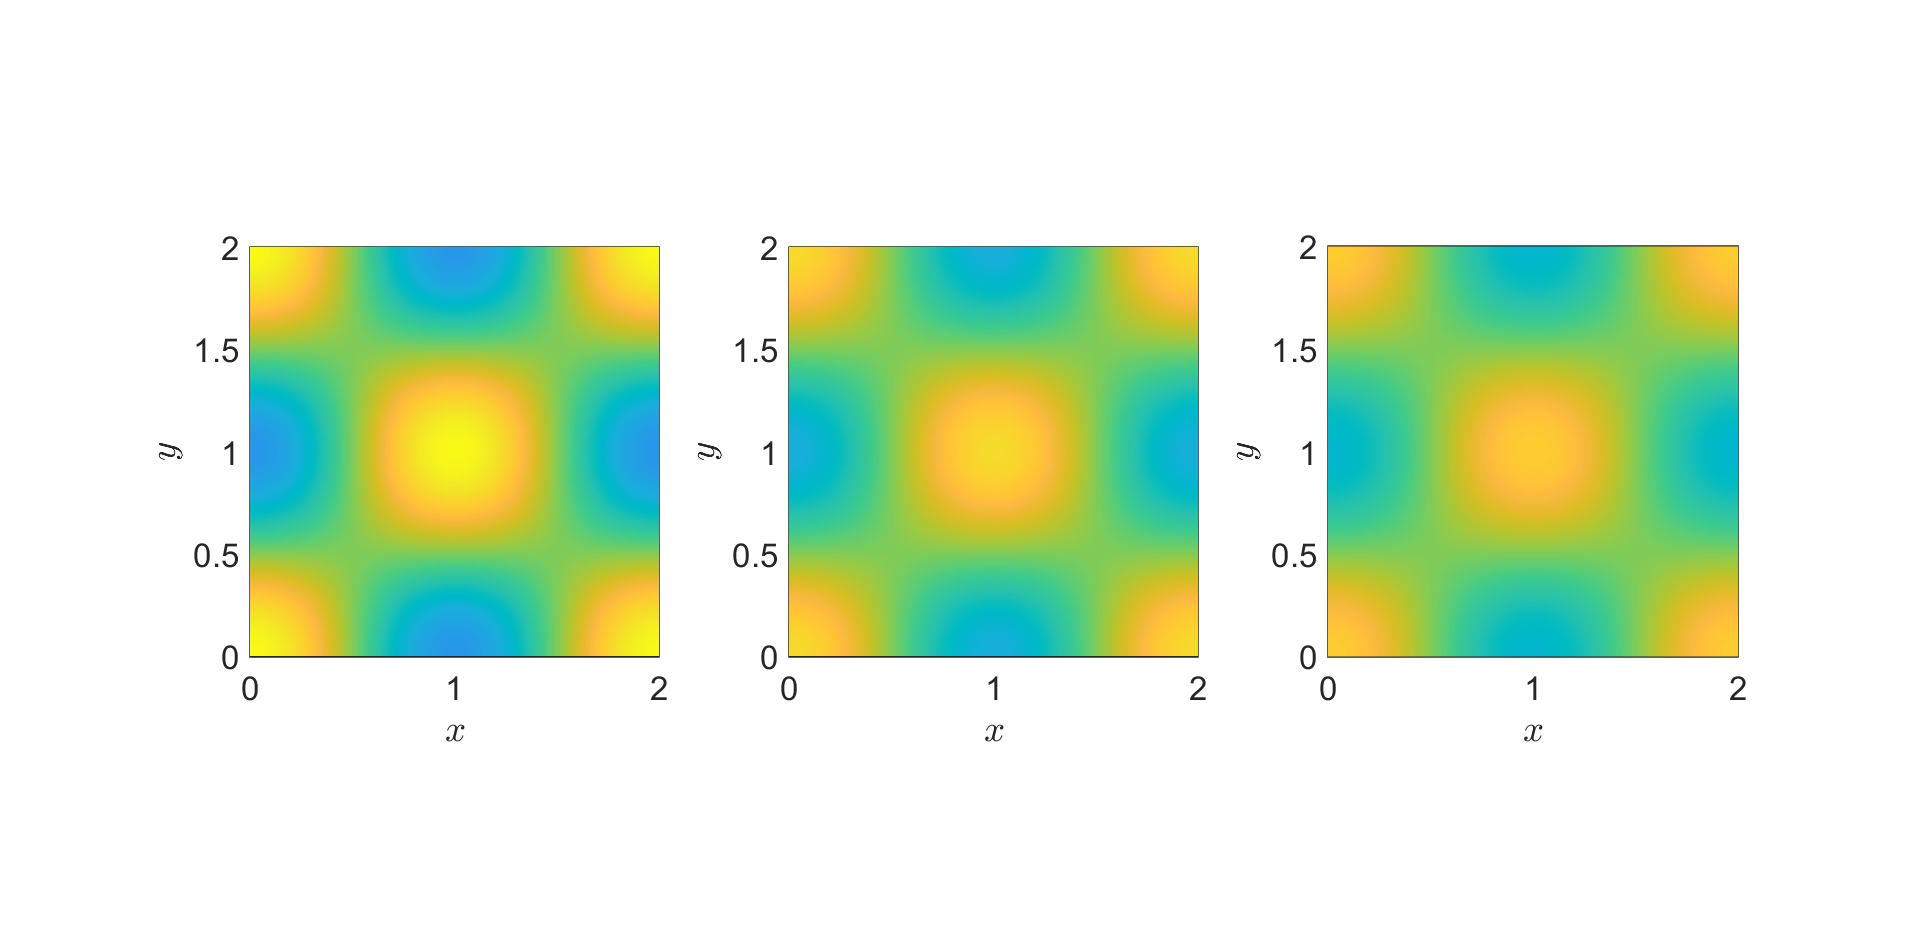
\includegraphics[scale=0.35]{boxExNoFlux.png}
	\caption{Exact solution on the box with no-flux boundary conditions.} 
	\label{F3b}
\end{figure}

\begin{figure}[h]
	\centering
	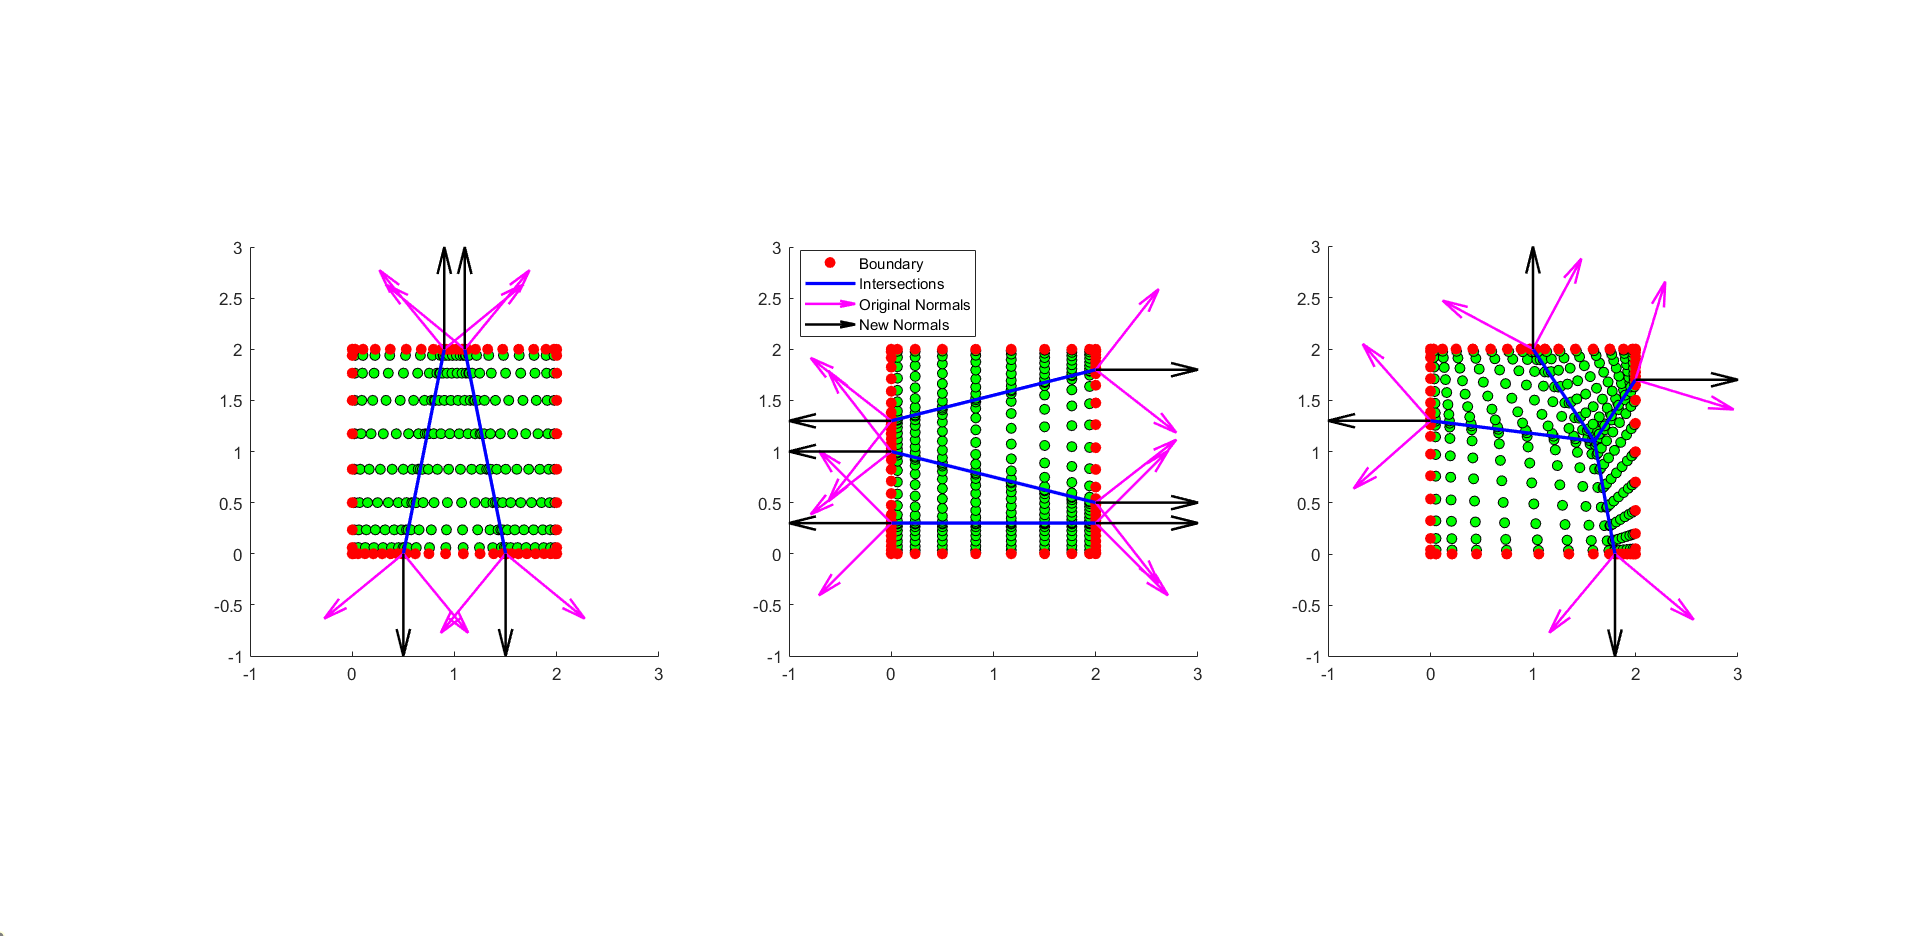
\includegraphics[scale=0.35]{NormalCorrected.png}
	\caption{Original, non-sensible normals are compared to new, customized normals.} 
	\label{FNorm}
\end{figure}

\begin{table}
\centering
\begin{tabular}{ | c | c | c | c | c | c | c |}
\hline
 & \multicolumn{2}{c|}{$N = 10$}  & \multicolumn{2}{c|}{$N = 20$}  & \multicolumn{2}{c|}{$N = 30$} \\
\hline
 & $\mathcal E_{Abs}$ & $\mathcal E_{Rel}$ & $\mathcal E_{Abs}$ & $\mathcal E_{Rel}$ & $\mathcal E_{Abs}$  & $\mathcal E_{Rel}$ \\
\hline
 a & $\numprint{1.0458e-2}$ & $\numprint{2.5230e-5}$ & $\numprint{2.8350e-7}$ & $\numprint{6.8623e-10}$ & $\numprint{2.6819e-7}$ & $\numprint{6.4918e-10}$ \\
 b & $\numprint{1.0178e-2}$ & $\numprint{1.7387e-5}$ & $\numprint{3.5488e-7}$ & $\numprint{6.0816e-10}$ & $\numprint{3.5538e-7}$ & $\numprint{6.0901e-10}$ \\
 c & $\numprint{7.1323e-2}$ & $\numprint{9.8994e-5}$ & $\numprint{7.0449e-3}$ & $\numprint{9.7842e-6}$ & $\numprint{2.6254e-3}$ & $\numprint{3.6463e-6}$ \\
 d & $\numprint{8.4906e-2}$ & $\numprint{1.0217e-4}$ & $\numprint{8.2570e-3}$ & $\numprint{9.9356e-6}$ & $\numprint{3.0338e-3}$ & $\numprint{3.6506e-6}$ \\
 e & $\numprint{5.6960e-3}$ & $\numprint{8.1264e-6}$ & $\numprint{4.3060e-7}$ & $\numprint{6.0669e-10}$ & $\numprint{4.3142e-7}$ & $\numprint{6.0784e-10}$ \\
 f & $\numprint{1.2934e-1}$ & $\numprint{1.5474e-4}$ & $\numprint{1.3465e-2}$ & $\numprint{1.6099e-5}$ & $\numprint{4.0715e-3}$ & $\numprint{4.8753e-6}$ \\
 g & $\numprint{8.7462e-6}$ & $\numprint{1.0753e-8}$ & $\numprint{5.1501e-7}$ & $\numprint{6.2332e-10}$ & $\numprint{5.1469e-7}$ & $\numprint{6.2294e-10}$ \\
\hline
\end{tabular}
\caption{Table No-Flux Exact Solution}
\label{Tab:NoFluxEx}
\end{table}
\begin{table}
\centering
\begin{tabular}{ | c | c | c | c | c | c | c |}
\hline
 & \multicolumn{2}{c|}{$N = 10$}  & \multicolumn{2}{c|}{$N = 20$}  & \multicolumn{2}{c|}{$N = 30$} \\
\hline
 & $\mathcal E_{Abs}$ & $\mathcal E_{Rel}$ & $\mathcal E_{Abs}$ & $\mathcal E_{Rel}$ & $\mathcal E_{Abs}$  & $\mathcal E_{Rel}$ \\
\hline
 c & $\numprint{1.8668e-2}$ & $\numprint{2.5911e-5}$ & $\numprint{4.5961e-7}$ & $\numprint{6.4023e-10}$ & $\numprint{4.5881e-7}$ & $\numprint{6.3911e-10}$ \\
 d & $\numprint{2.4277e-2}$ & $\numprint{2.9194e-5}$ & $\numprint{5.2874e-7}$ & $\numprint{6.3810e-10}$ & $\numprint{5.2815e-7}$ & $\numprint{6.3740e-10}$ \\
 f & $\numprint{2.1887e-3}$ & $\numprint{2.6634e-6}$ & $\numprint{5.3703e-7}$ & $\numprint{6.3964e-10}$ & $\numprint{5.3681e-7}$ & $\numprint{6.3938e-10}$ \\
\hline
\end{tabular}
\caption{Table No-Flux Exact Solution with Corrected Normal Vectors at Intersections}
\label{Tab:NoFluxCorr}
\end{table}
\subsection*{Forward Problems on multishapes}
We first consider a forward problem on the different discretizations of the box, see Figure \ref{F2}. We compare the results of the discretized boxes with the result for box (a) with large $N$.
We choose the initial condition for $\rho$ to be
\begin{align*}
	\rho_0 = \exp(-2((y_1 - 0.7 )^2 + (y_2 - 0.2)^2)),
\end{align*}
and impose a constant flow of strength $0.8$ acting upward.
We choose $N = 10$, $N = 20$ and $N = 30$ as before. The errors are displayed in Table \ref{Tab:FWProbBox} and the result can be seen in Figure \ref{FFW1}. 
%
%\begin{table}
%	\caption{Errors (compared to whole box with $N = 50$) for different discretizations of the box}
%	\begin{tabular}{ ||c| c| c| c| c| c| c|| }
%		\hline
%		\hline
%		& b & c & d & e & f & g\\ 
%		\hline
%		Abs. Error, $N =20$& $0.0129$ & $0.0194$ & $0.0337$& $0.032$&  $ 0.0165$ & $0.0099$ \\  
%		Rel. Error, $N =20$& $0.001$& $0.0025$ & $0.0024$ & $0.0025$& $0.0019$  & $0.0007$ \\
%		Abs. Error, $N =30$& $0.0054$ & $0.0078$ & $0.0137$ &$0.0134$&$0.0064$& $0.0026$\\  
%		Rel. Error, $N =30$ & $0.0003$& $0.0007$ &$0.0006$ &$0.0007$&$0.0005$& $0.0001$\\
%		\hline
%		\hline
%	\end{tabular}
%	\label{Tab3:ErrorsFWBox}
%\end{table}
\begin{figure}[h]
	\centering
	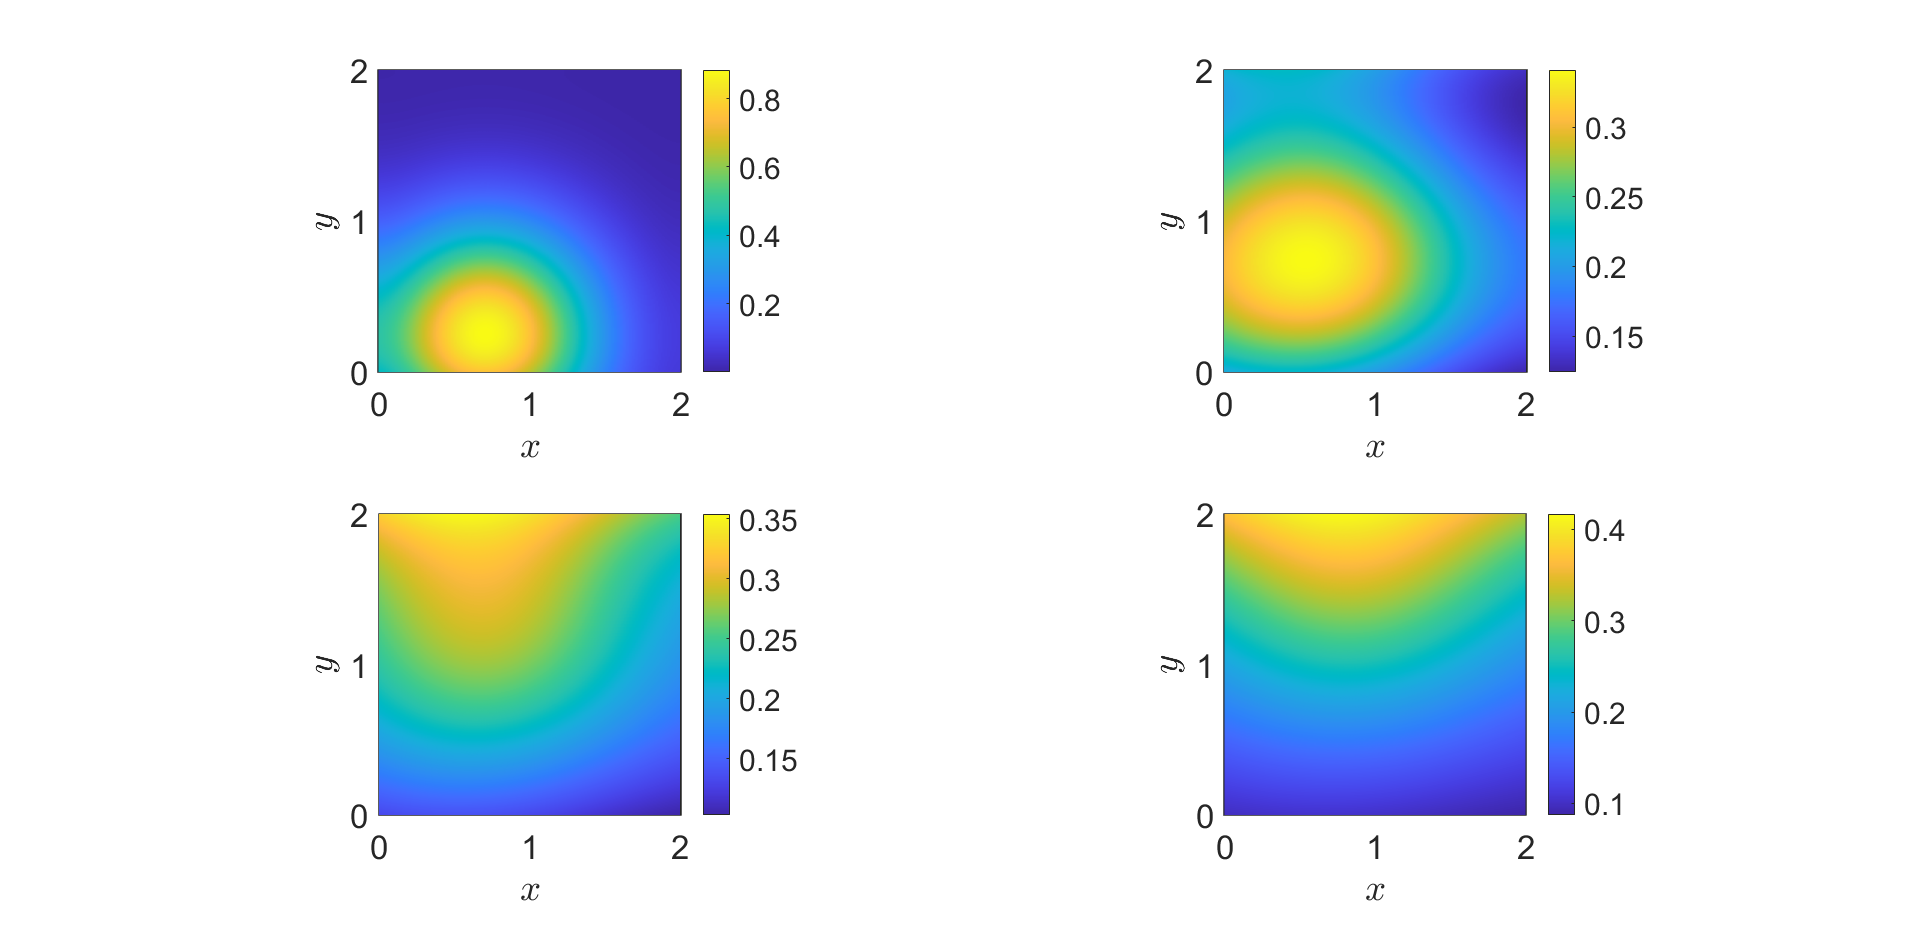
\includegraphics[scale=0.35]{FWBox.png}
	\caption{Forward Example on box discretizations} 
	\label{FFW1}
\end{figure}


We follow the same idea, but now consider the wedge discretizations, see Figure \ref{F4}. We choose the initial condition for $\rho$ to be
\begin{align*}
	\rho_0 = \exp(-2((y_1 - 1.5 )^2 + (y_2 - 4.5)^2)),
\end{align*}
and impose a constant flow of strength $3$ acting from left to right, along the angular direction.
We choose $N = 20$ and $N = 30$. The errors are displayed in Table \ref{Tab:FWProbWedge} and the result can be seen in Figure \ref{FFW2}. 

%\begin{table}
%	\caption{Errors (compared to whole wedge (h) ) for different discretization (into two and three shapes) of the wedge}
%	\begin{tabular}{ ||c| c| c| c|| }
%		\hline
%		\hline
%		& i & j &k\\ 
%		\hline
%		Abs. Error, $N =20$& $0.0233 $ & $0.0750 $ & $0.0189 $ \\  
%		Rel. Error, $N =20$& $0.0026 $& $0.0068 $ &$0.0013 $ \\
%		Abs. Error, $N =30$& $0.0071 $ & $0.0316 $ & $0.0113 $  \\  
%		Rel. Error, $N =30$ & $0.0005 $& $0.0019 $ &$ 0.0005$  \\
%		\hline
%		\hline
%	\end{tabular}
%	\label{Tab4:ErrorsFWWedge}
%\end{table}
\begin{figure}[h]
	\centering
	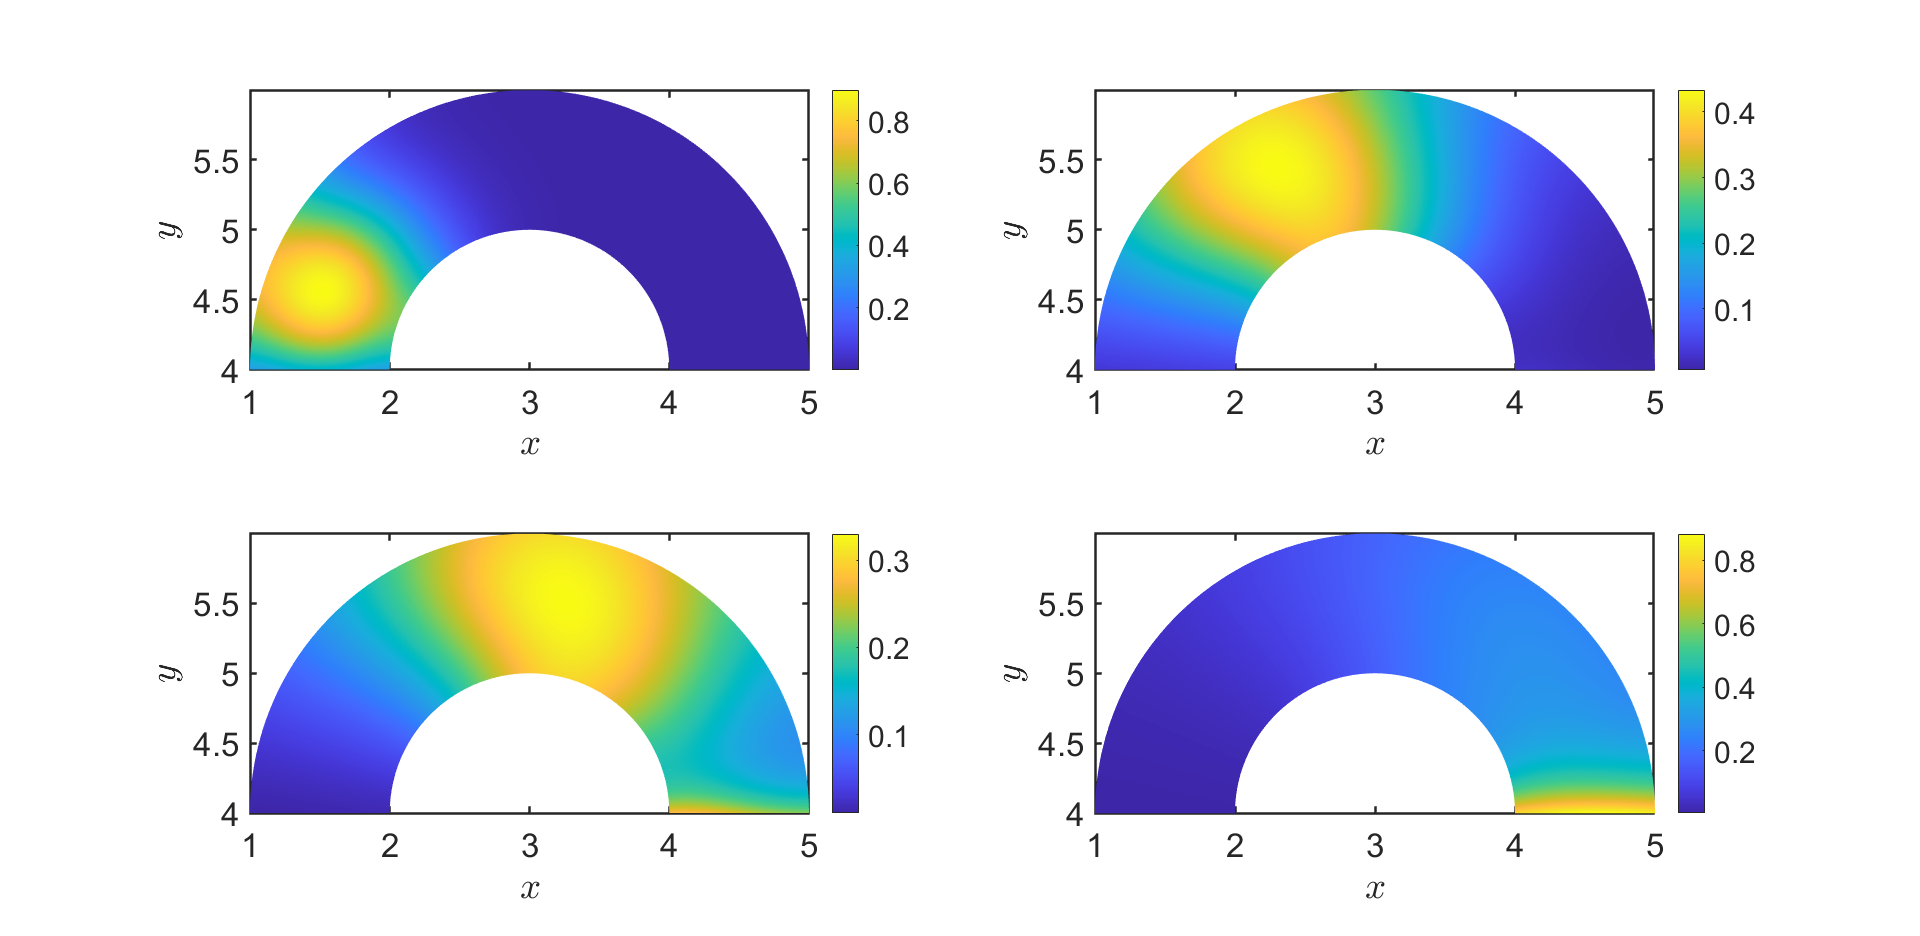
\includegraphics[scale=0.35]{FWWedge.png}
	\caption{Forward Example on wedge discretizations} 
	\label{FFW2}
\end{figure}



Finally, two more complex multishape examples are considered.
The first of these examples is solving an advection diffusion problem on a multishape consisting of two quadrilaterals and two wedges, with constant velocity of strength ten. The initial condition for this problem is:
 \begin{align*}
 	\rho_0 = \exp( -2(y_1 -0.5)^2 - 2 (y_2 + 1)^2).
 \end{align*}
The result, evaluated for $N= 20$ on each shape, can be seen in Figure \ref{F8}.

\begin{figure}[h]
	\centering
	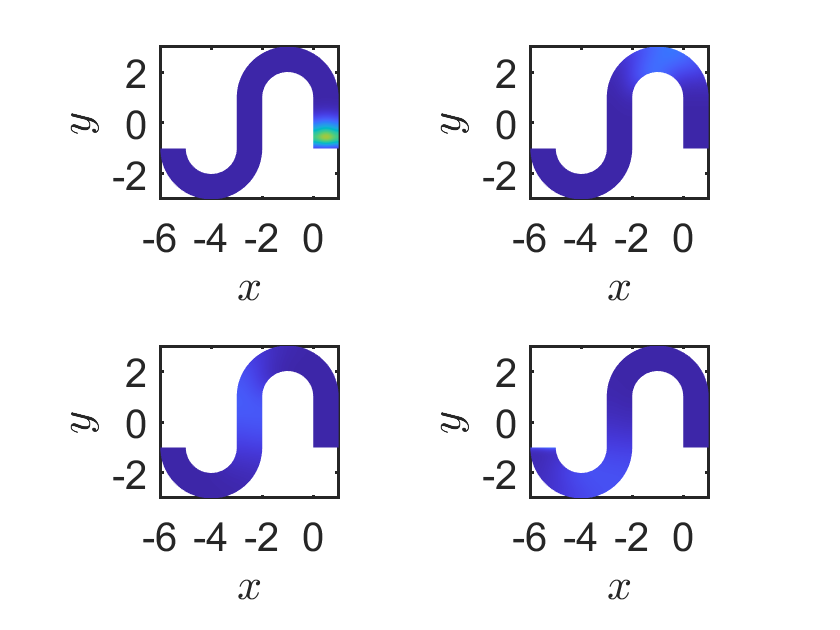
\includegraphics[scale=0.35]{ex1.png}
	\caption{Forward Problem 1, different colour scale for each plot to highlight particle mass location}
	\label{F8}
\end{figure}

In a second example, the velocity is of strength $5$ and the initial condition is:
 \begin{align*}
	\rho_0 = \exp( -2(y_1 -0.5)^2 - 2 (y_2 - 1.5)^2).
\end{align*}
The result, which is computed on a multishape made up of four quadrilaterals into a channel, can be seen in Figure \ref{F9}.

\begin{figure}[h]
	\centering
	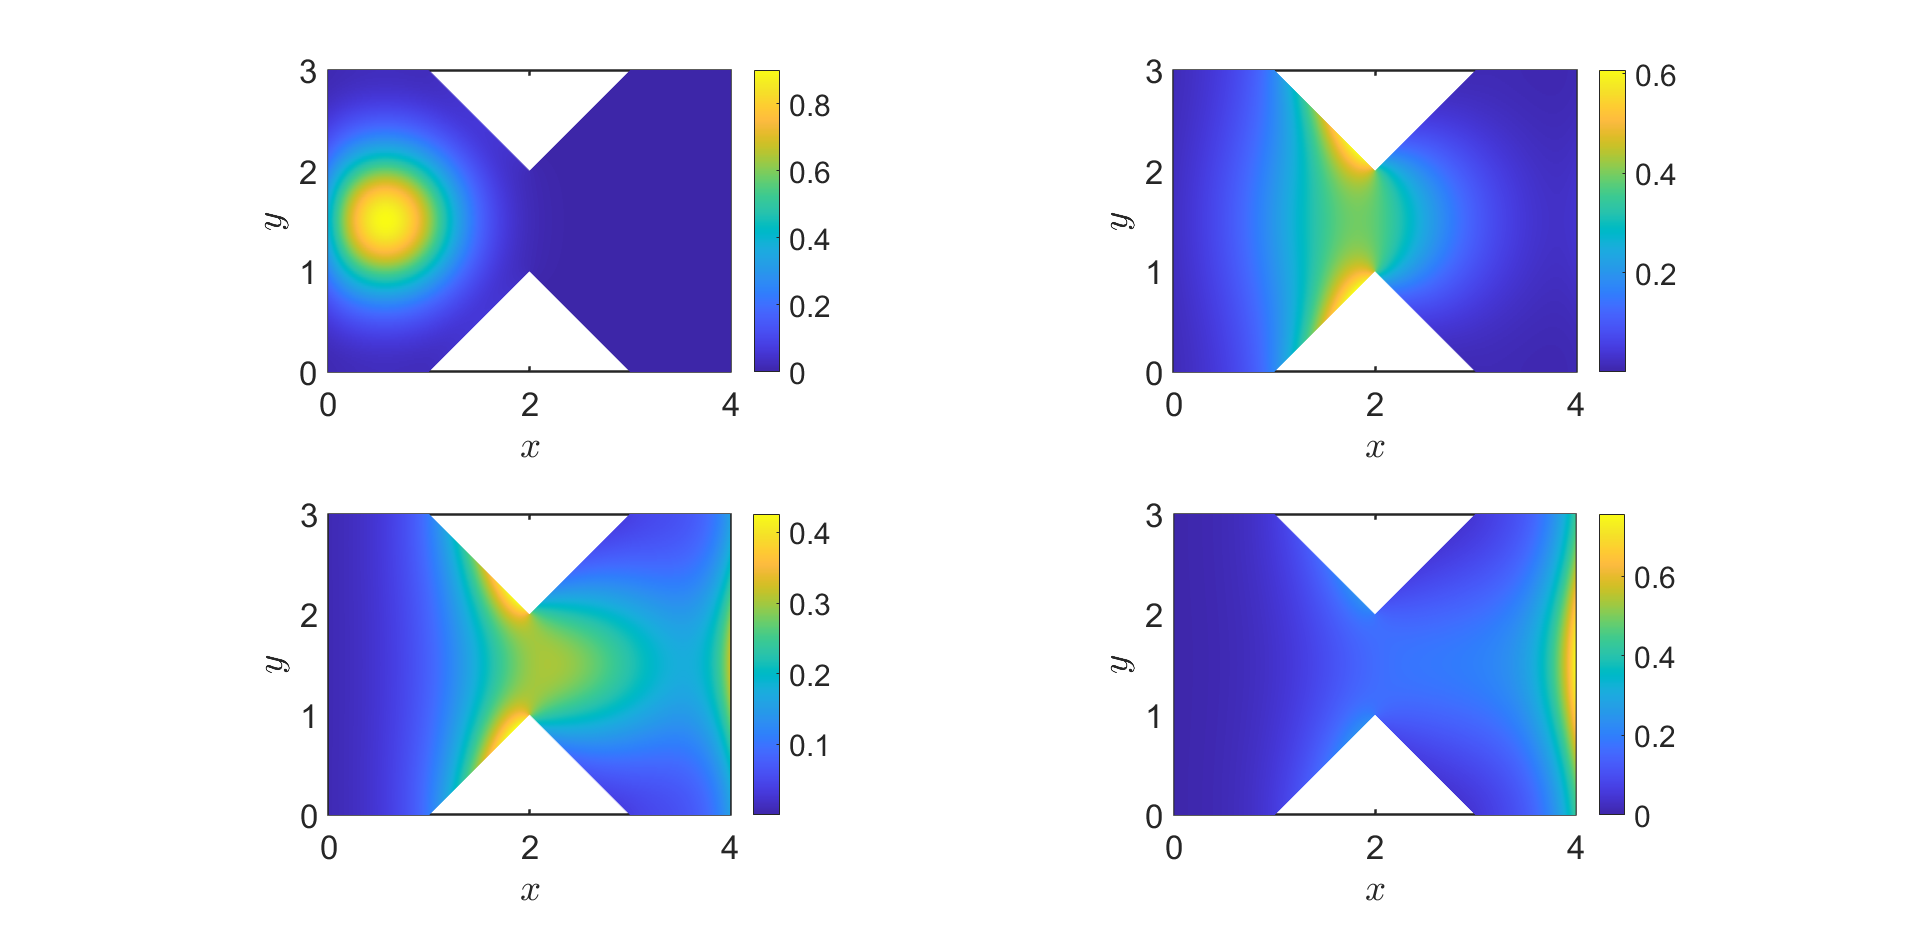
\includegraphics[scale=0.35]{ex2.png}
	\caption{Forward Problem 2, different colour scale for each plot to highlight particle mass location}
	\label{F9}
\end{figure}

In Table \ref{Tab:Example12} the solution to these two examples is evaluated with $N = 30$ and compared to the solution evaluated with $N = 10$, $N = 15$ and $N = 20$, using the same error measure as before. We can see that the solution converges with the number of points. It is especially noticeable for Example 1, that $N = 10$ does not give a reliable solution at all, while $N = 15$ provides a solution that is reasonably close to the one with $N = 30$. The reason that Example 1 is much more sensitive to the number of points than Example 2 could be that it contains polar shapes. As discussed in Section \ref{sec:ValidationDiffIntetc}, for accurate interpolation of the wedge, the angular direction needs more points than the radial direction, and in particular was not very accurate with $N = 10$ in the angular direction.




\begin{table}
\centering
\begin{tabular}{ | c | c | c | c | c | c | c |}
\hline
 & \multicolumn{2}{c|}{$N = 10$}  & \multicolumn{2}{c|}{$N = 20$}  & \multicolumn{2}{c|}{$N = 30$} \\
\hline
 & $\mathcal E_{Abs}$ & $\mathcal E_{Rel}$ & $\mathcal E_{Abs}$ & $\mathcal E_{Rel}$ & $\mathcal E_{Abs}$  & $\mathcal E_{Rel}$ \\
\hline
 b & $\numprint{6.8019e-2}$ & $\numprint{1.7873e-2}$ & $\numprint{1.9441e-2}$ & $\numprint{2.4954e-3}$ & $\numprint{7.8355e-3}$ & $\numprint{6.6545e-4}$ \\
 c & $\numprint{4.5117e-2}$ & $\numprint{6.9628e-3}$ & $\numprint{1.2944e-2}$ & $\numprint{9.9990e-4}$ & $\numprint{5.3658e-3}$ & $\numprint{2.7644e-4}$ \\
 d & $\numprint{1.1864e-1}$ & $\numprint{1.7013e-2}$ & $\numprint{3.3678e-2}$ & $\numprint{2.3638e-3}$ & $\numprint{1.3708e-2}$ & $\numprint{6.3705e-4}$ \\
 e & $\numprint{1.2516e-1}$ & $\numprint{1.9815e-2}$ & $\numprint{3.1984e-2}$ & $\numprint{2.5133e-3}$ & $\numprint{1.3367e-2}$ & $\numprint{6.9858e-4}$ \\
 f & $\numprint{5.8413e-2}$ & $\numprint{1.4025e-2}$ & $\numprint{1.6467e-2}$ & $\numprint{1.9292e-3}$ & $\numprint{6.3541e-3}$ & $\numprint{4.9237e-4}$ \\
 g & $\numprint{4.0532e-2}$ & $\numprint{5.7827e-3}$ & $\numprint{9.9059e-3}$ & $\numprint{7.0226e-4}$ & $\numprint{2.5623e-3}$ & $\numprint{1.2085e-4}$ \\
\hline
\end{tabular}
\caption{Table Forward Problem on Box}
\label{Tab:FWProbBox}
\end{table}
\begin{table}
\centering
\begin{tabular}{ | c | c | c | c | c | c | c |}
\hline
 & \multicolumn{2}{c|}{$N = 10$}  & \multicolumn{2}{c|}{$N = 20$}  & \multicolumn{2}{c|}{$N = 30$} \\
\hline
 & $\mathcal E_{Abs}$ & $\mathcal E_{Rel}$ & $\mathcal E_{Abs}$ & $\mathcal E_{Rel}$ & $\mathcal E_{Abs}$  & $\mathcal E_{Rel}$ \\
\hline
 i & $\numprint{8.1092e-2}$ & $\numprint{1.8792e-2}$ & $\numprint{2.3281e-2}$ & $\numprint{2.6395e-3}$ & $\numprint{7.0628e-3}$ & $\numprint{5.3006e-4}$ \\
 j & $\numprint{2.8569e-1}$ & $\numprint{5.2137e-2}$ & $\numprint{7.5030e-2}$ & $\numprint{6.8191e-3}$ & $\numprint{3.1628e-2}$ & $\numprint{1.9130e-3}$ \\
 k & $\numprint{7.0422e-2}$ & $\numprint{9.7166e-3}$ & $\numprint{1.8884e-2}$ & $\numprint{1.2887e-3}$ & $\numprint{1.1284e-2}$ & $\numprint{5.1154e-4}$ \\
\hline
\end{tabular}
\caption{Table Forward Problem on Wedge}
\label{Tab:FWProbWedge}
\end{table}
\begin{table}
\centering
\begin{tabular}{ | c | c | c | c | c | c | c |}
\hline
 & \multicolumn{2}{c|}{$N = 10$}  & \multicolumn{2}{c|}{$N = 15$}  & \multicolumn{2}{c|}{$N = 20$} \\
\hline
 & $\mathcal E_{Abs}$ & $\mathcal E_{Rel}$ & $\mathcal E_{Abs}$ & $\mathcal E_{Rel}$ & $\mathcal E_{Abs}$  & $\mathcal E_{Rel}$ \\
\hline
 Ex1 & $\numprint{1.7380e+121}$ & $\numprint{1.3801e+121}$ & $\numprint{2.9942e-1}$ & $\numprint{5.0366e-2}$ & $\numprint{1.5166e-1}$ & $\numprint{1.7141e-2}$ \\
 Ex2 & $\numprint{3.1819e-2}$ & $\numprint{8.9836e-3}$ & $\numprint{1.4655e-2}$ & $\numprint{2.2034e-3}$ & $\numprint{9.7279e-3}$ & $\numprint{1.0914e-3}$ \\
\hline
\end{tabular}
\caption{Table Forward Examples 1 and 2}
\label{Tab:Example12}
\end{table}
